\documentclass[
    corpo=12pt,
    oneside,
    evenboxes,
    tipotesi=triennale,
    stile=classica,
    oldstyle,
    autoretitolo,
    greek,
]{toptesi}
\usepackage[utf8]{inputenc}
\usepackage[T1]{fontenc}
\usepackage{lmodern}
\usepackage{hyperref}
\usepackage{setspace}
\usepackage{verbatim}
\usepackage{pgfplots}
\usepackage{graphicx}
\usepackage{subfig}
\usepackage{amsmath}
\usepackage{eurosym}
\usepackage{enumerate}
\usepackage{booktabs}
\usepackage{tabularx}
\onehalfspacing

\hypersetup{
    pdfpagemode={UseOutlines},
    bookmarksopen,
    pdfstartview={FitH},
    colorlinks,
    linkcolor={blue},
    citecolor={blue},
    urlcolor={blue}
  }
\usepackage{lipsum}

\begin{document}\errorcontextlines=9

\begin{ThesisTitlePage}
    \ateneo{Universit\`a degli Studi di Torino}
    \StrutturaDi{Dipartimento di Management}
    \struttura[]{}
    \NomeElaborato{Tesi di laurea triennale}
    \titolo{Lo stato di salute del Calcio pre e post COVID-19}
    \sottotitolo{Fair Play Fiananziario e Superlega}     
    \corsodistudi{Management dell'Informazione e della Comunicazione Aziendale}
    \candidato{Riccardo \textsc{Borgo}}
    \relatore{prof.ssa ~Simona \textsc{Alfiero}}
    \sedutadilaurea{\textsc{Anno~accademico} 2021-2022}
    \logosede{img/Unito-logo, img/logo_saa.jpeg}
\end{ThesisTitlePage}

\figurespagetrue\tablespagetrue
\indici

\mainmatter
\begin{interlinea}{1.5}

\part{Parte Prima}
\chapter{Introduzione generale}
Durante lo sviluppo di questa trattazione si andrà ad analizzare lo "stato di salute" del calcio europeo prima e dopo 
l'avvento della pandemia COVID19 che ha sicuramente stravolto la vita di tutti ed ha sicuramente arrecato non pochi danni 
economici al mondo, compreso quello del calcio.\newline
Il primo capitolo verter\'a principalmente sull'analisi della situazione economica pre-pandemia, per permettere di delineare una situazione
completa e capire se anche prima del 2020 esistessero gi\'a dei problemi nell'economia del calcio. Per primo verr\'a approfondito lo scenario
globale all'interno dei 5 pi\'u importanti Paesi Europei: Italia, Francia, Germania, Spagna e Inghilterra. Essi sono le realt\'a pi\'u 
affermate e potenti all'interno del sistema calcio, nonstante negli ultimi anni stiano crescendo molto anche altri campionati come per esempio
quello Olandese e altri dall'Est Europa. Questa prima parte avr\'a come argomento due indicatori principali: \textbf{Risultato Economico 2019} 
con la sua relativa scomposizione in \textbf{costi} e \textbf{ricavi} e gli \textbf{stipendi}. Questi due elementi
permettono di generare un'opinione trasversale e completa della situazione. Verrà mostrato come non in tutti 
si riesca ad arrivare ad un risultati positivo, andando quindi a rendere in qualche modo 
"unico" ogni campionato e la sua relativa Federazione. Le Federazioni (uniche per ogni Stato) hanno il compito
comune di organizzare i campionati nazionali e designare gli arbitri per i vari incontri. Oltre a questo compito pi\'u di tipo
organizzativo le varie Federazioni hanno il dovere di garantire un accesso libero ed universale al gioco del calcio, senza distinzioni
di genere ed etnia. Questi due compiti \'e possibile estrapolarli dagli 11 punti contenenti i valori che la UEFA
\footnote{Wikipedia: Union of European Football Associations, raggruppa tutte le Federazioni dei vari stati Europei e non} vuole
trasmettere tramite la sua attivit\'a\footnote{Wikpedia: https://it.wikipedia.org/wiki/Union\_of\_European\_Football\_Associations, I Valori UEFA}.\newline
La seconda parte del primo capitolo analizzer\'a la situazione economica, finanziaria e patrimoniale sempre antecedente all'anno 2020 di alcune delle più 
importanti e storiche societ\`a di tutto il panorama europeo: Juventus per quanto riguarda l'Italia, Paris Saint Germain per quanto riguarda la 
Francia, Bayern Monaco per la Germania, Manchester City per l'Inghiterra e il Barcellona per la Spagna. I punti principali dell'analisi riguarderanno: 
Analisi dei ricavi, Analisi della liquidit\'a, Analisi della solidit\'a e Analisi della redditivit\'a in modo da 
poter fare una verifica a 360° di tutti i vari settori economici. La scelta \'e caduta su queste societ\'a perch\'e, per un motivo o per un altro, sono state 
al centro di problematiche o inchieste legate al \emph{Financial Fair Play}.\newline
Il secondo capitolo si occuper\'a invece della presentazione e dell'analisi in modo dettagliato delle varie regole imposte con il
\textbf{Financial Fair Play} tramite i vari capitoli del documento. Il punto cruciale di questo capitolo sar\'a dimostrare come, non sempre, 
tutte le societ\'a siano state trattate allo stesso modo, evitando a volte sanzioni pi\'u che meritate\newline
Il terzo capitolo, ed ultimo capitolo, analizzer\'a l'impatto mediatico, non prima di aver presentato tutti i dati tecnici, di una delle ultime novità 
del mondo del calcio: la \textbf{Superlega}: il nuovo modello che punta a rivoluzionare il mondo del calcio, per cercare di uscire da questa spirale di debiti
e fallimenti per cercare quindi di creare un nuovo inizio. Verr\'a mostrato in seguito se il progetto ha effettivamente preso piede all'interno del mondo del calcio 
e se è riuscito a smuovere qualcosa, portando agli occhi di tutti l'insostenibilità del modello attuale.\newline
In chiusura si cercherà di determinare se i rimedi proposti dalle autorità del mondo del calcio siano stati sufficienti ad eliminare tutte le criticità presenti e 
sopratutto evidenziare l'impatto economico di questi rimedi.\\
Riuscir\'a la Superlega ad acquistare credibilità e ad affermarsi come nuovo modello, capace di risollevare il calcio?

\part{Parte Seconda}
\chapter{Situazione economica Europea pre-pandemia COVID19}
\section{Analisi generale delle diverse realt\'a Europee}
Il primo paese preso in esame \'e l'\textbf{Italia}, il quale presenta una situazione decisamente non ottimale. La gestione del sistema calcio 
\'e affidata alla FIGC\footnote{Federazione Italiana Giuoco Calcio} che si è rivelata nel corso degli anni non irresistibile nella gestione economica
di tutto il sistema ed \'e stata addirittura legata ad affari illeciti: il pi\'u eclatante sicuramente il caso \emph{Calciopoli} 
datato 2006 che ancora oggi non ha prodotto un vero colpevole ma ha comunque portato alla dimissione dell'allora Presidente e 
Vicepresidente Franco Carraro e Innocenzo Mazzini\footnote{Wikipedia: https://it.wikipedia.org/wiki/Calciopoli}.
Tornando all'analisi prettamente economica, la sezione dei \textbf{Ricavi} a partire dalla stagione 2013/2014 ha sempre registrato un valore 
in crecita, passando da 2.625mln€ nel 2013/2014 a 3.854mln€ nel 2018/2019 (incremento del 46\%)\footnote{FIGC: https://www.figc.it/it/federazione/federazione-trasparente/reportcalcio/}. 
Anche se i dati riportano un valore complessivamente in linea con la maggior parte degli altri Paesi, il fatto che non rassicura \'e che non
ci sia mai stata la capacit\'a di avere un valore di ricavi che superasse quello dei costi. La voce che abbatte maggiormente il valore 
della produzione sono gli ammortamenti che, nel caso del calcio, 
si riferiscono al costo del cartellino dei calciatori (costo storico) e il loro relativo contratto (vita utile). L'aumento di questa voce
non sarebbe, tuttavia, un aspetto negativo dato che spiega come le societ\'a vogliano investire in risorse nuove per il miglioramento delle
rose. Il problema sorge per\'o se non si ottengono risultati sul campo, sopratutto quello internazionale che costituisce la maggior parte
degli incassi dei club. A prova di questo l'ultimo successo in campo 
internazionele da parte di una squadra italiana risale al 2010 con la vittoria della Champions League da parte dell'Inter e, a parte
le due finali raggiunte dalla Juventus, non ci sono stati altri traguardi degni di nota da parte dei team italiani in Europa.\newline
Passando invece all'argomento \textbf{stipendi} la FIGC non fornisce un resoconto dettagliato riguardo gli stipendi dei tesserati durante l'anno
come accade per altri Paesi; l'unico spunto di analisi pu\'o essere estrapolato dall'approfondimento sulle voci di costo all'interno del report.
Quest'ultima non permette di creare un'opinione a 360° dell'argomento, poich\'e se si osserva solamente il grafico ripreso 
dalla figura \ref{figA} si potrebbe constatare come non ci siano particolari debolezze dato che il peso degli stipendi rimane costante sui vari anni. 
Il problema sorge osservando la figura accanto \ref{figB}\footnote{Ultimo Uomo: https://www.ultimouomo.com/guida-ai-monte-ingaggi-della-serie-a-2018-19/} 
che mostra come due societ\'a abbiano abbattuto il tetto dei 100mln€ di ingaggio per i calciatori e di come altre 3 societ\'a ci 
siano andate molto vicino. Complessivamente troviamo un generale aumento degli stipendi che per\'o non viene bilaniato con bassissimi introiti 
dalle competizioni internazionali.\newline
\begin{figure}
    \centering
    \subfloat[][Composizione dei costi all'interno del sistema calcio italiano]
    {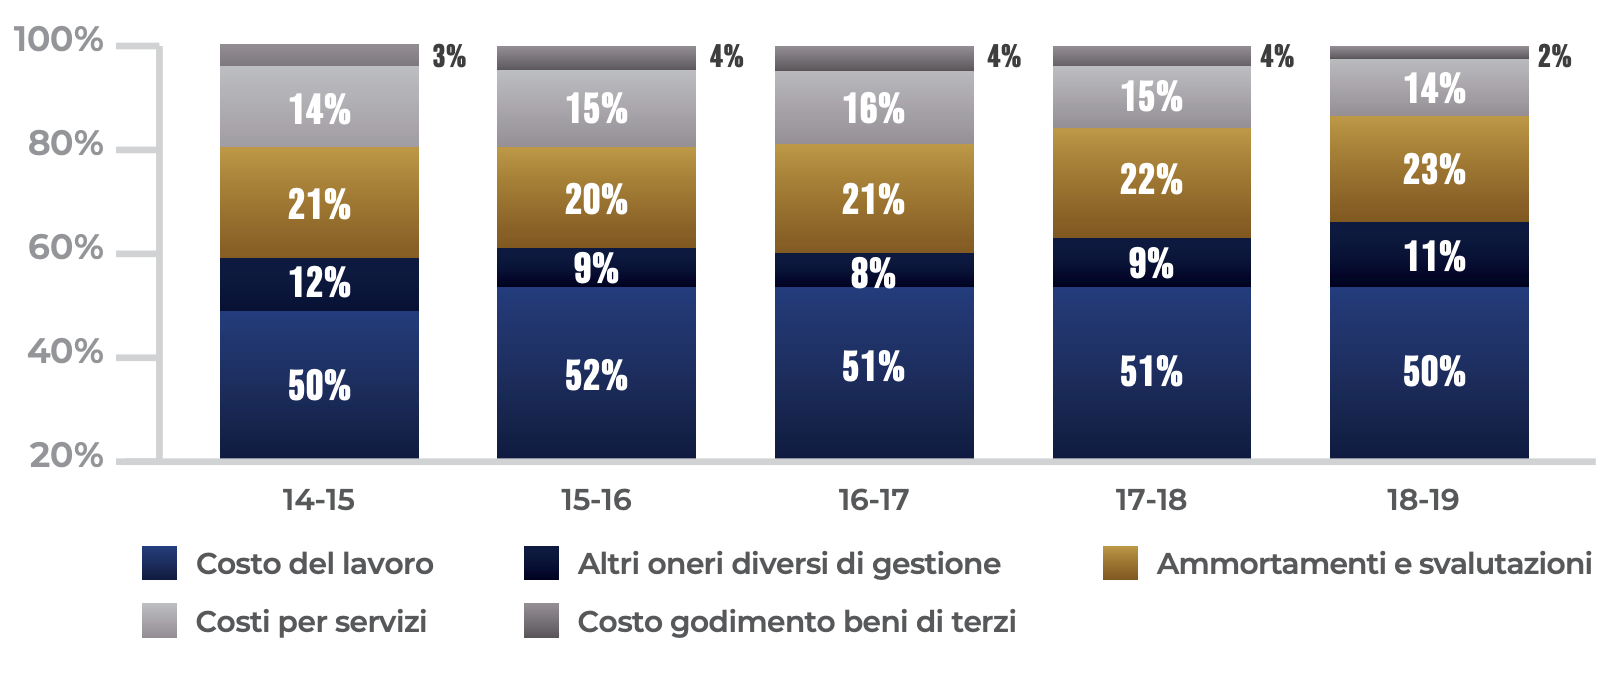
\includegraphics[width=.55\textwidth]{img/wage_serieA.png} \label{figA}} \quad
    \subfloat[][Confronto stipendi Serie A 17/18 e 18/19]
    {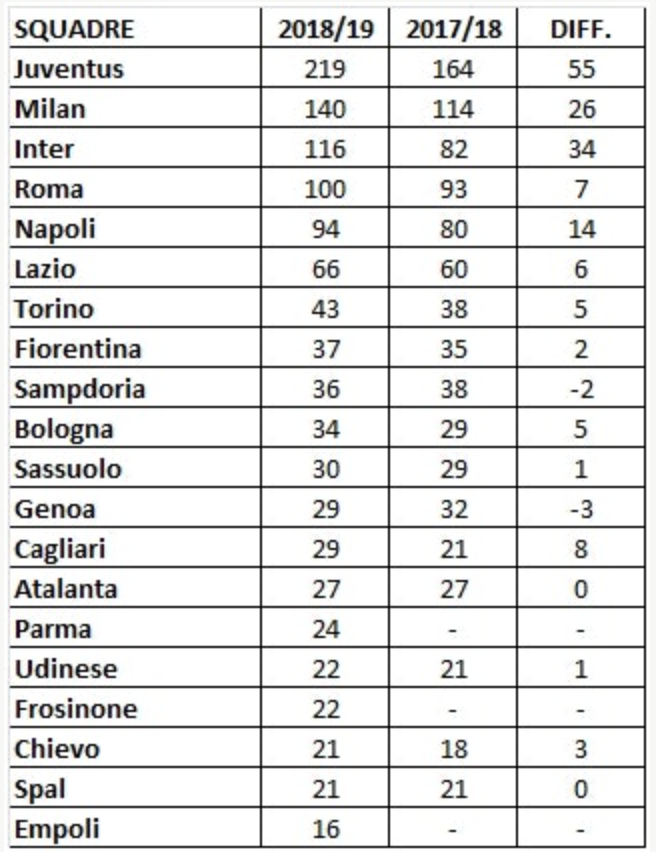
\includegraphics[width=.25\textwidth]{img/diff_wage_serieA.png} \label{figB}}
    \caption{Situazione \emph{Costo del Lavoro} all'interno del calcio italiano}
    \label{wage_serieA}  
\end{figure}\newline
Per quanto riguarda invece la \textbf{Francia}, l'organizzazione che si occupa del monitoraggio e la supervisione dei conti 
delle società calcistiche è la DNCG\footnote{Direction Nationale du Contrôle de Gestion}. Essa 
pubblica ogni stagione un report riassuntivo per quanto riguarda la Ligue 1 e la Ligue 2 (i primi due campionati) ed una
relazione relativa ad ogni singolo club dei due campionati. Tutti i dati di seguito riportati sono stati reperiti dai singoli
report annuali pubblicati\footnote{https://www.lfp.fr/dncg/rapports} \newline 
La perdita registrata nella stagione 18/19 che ammontava a 126mln€ \'e la seconda in termini di importanza a partire dal 2013/2014,
il motivo principale che spiega questa discesa cos\'i decisa \'e da attribuirsi ad un aumento delle entrate (\emph{Income})
da 304mln€ nel 17/18 a 316mln€ nel 18/19, che per\'o non riesce a contrastare l'aumento pi\'u elevato
delle spese (\emph{Expenses}) sopratutto nella sezione dedicata agli stipendi di giocatori e commissioni degli agenti 
dove troviamo un aumento rispetto all'anno precedente di 9mln€.\newline
Il secondo indicatore che viene preso in considerazione \'e chiamato \textbf{Payroll}, termine indicante la somma dei vari stipendi
dei dipendenti di un club. Nonostante un Payroll, almeno per quanto riguarda le squadre qualificate per la UCL\footnote{Uefa Champions League}, in linea con gli
altri campionati (147 mln€ nella Premier League inglese\footnote{Calcolo personale utilizzando i dati da https://www.spotrac.com/epl/payroll/}),
i risultati ottenuti nelle competizioni internazionali non sono state all'altezza: nella stagione 2018/2019 sono presenti 3 squadre 
all'interno della fase a gironi della massima competizione europea: Monaco, Paris Saint Germain e Olympique Lione. La prima si 
posizione ultima nel gruppo A, la seconda (da cui gli esperti e i sostenitori si aspettano grandi risultati, visti i milioni di euro 
spesi ogni anno) viene eliminata agli ottavi di finale e infine la terza viene anch'essa eliminata agli ottavi di finale. Questo scenario
si ripete mediamente ogni anno, in aggiunta, se si vuole trovare una squadra francese vincitrice della massima competizione europea 
dobbiamo tornare indietro alla stagione 1992/1993 con l'Olympique Marsiglia. La figura \ref{stipendi_ligue1} permette di capire, 
oltre alla disparit\'a di risorse in possesso dei club in Francia, anche il livello di spesa dei club per gli stipendi, che come \'e stato detto in precedenza non viaggia 
di pari passo ai traguardi interazionali.\newline
\begin{figure}
    \centering
    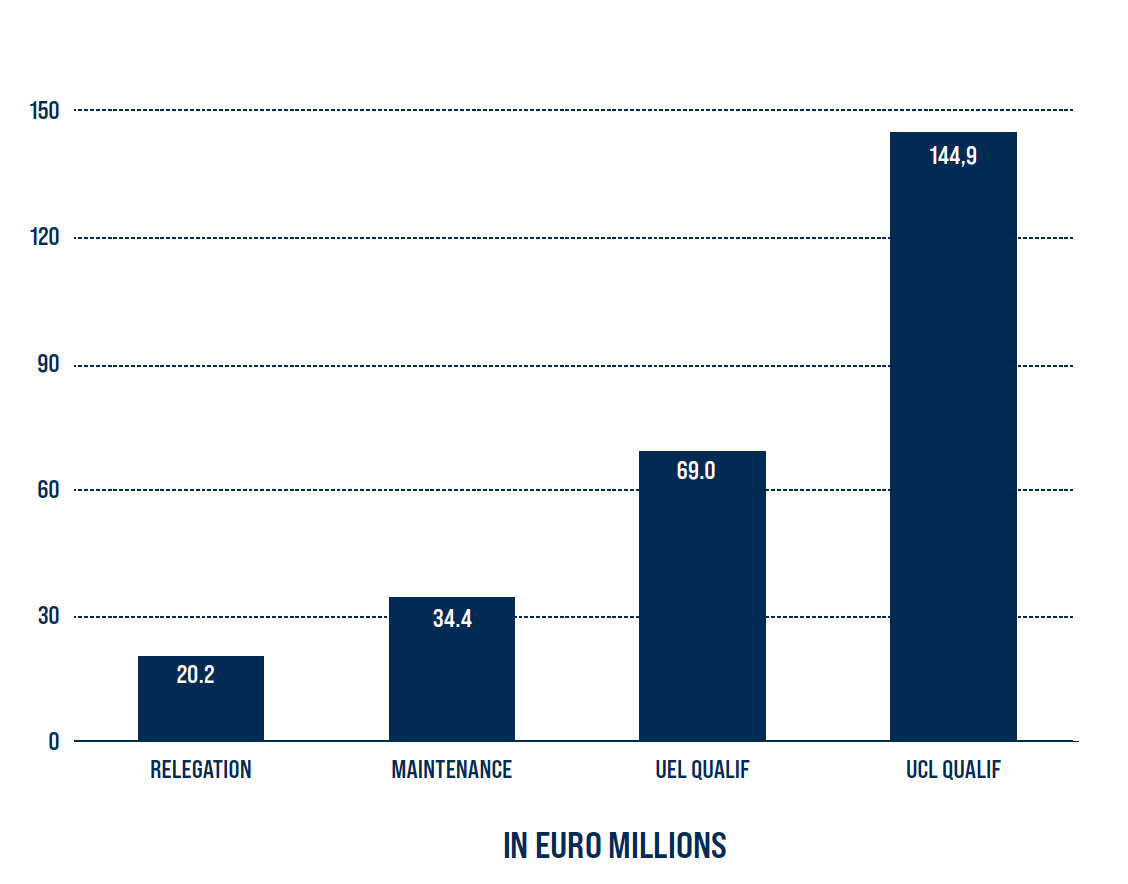
\includegraphics[scale=0.5]{img/stipendi_ligue1.png}
    \caption{Stipendi Ligue 1 a seconda del piazzamento in classifica}
    \label{stipendi_ligue1}
\end{figure}
Riprendendo l'ultimo indicatore analizzato e collegandolo al primo \'e possibile sviluppare uno scenario simile all'Italia, dove
i grandi investimenti non portano al successo assicurato e quindi ad un ritorno concreto. Queste grosse somme che escono dalle casse 
dei club che non vedono un ritorno portano un danno a tutto il campionato, all'interno del quale aumenta il gap tecnico tra le diverse squadre dello
stesso campionato mentre dall'altro, in campo internazionale, non si ottengono risultati non ricevendo quindi premi da sponsor e organizzatori.
Tutto questo circolarit\'a non fa' altro che danneggiare il sistema calcio francese facendogli perdere valore e \emph{appeal}.\newline
Il terzo Paese e di conseguenza ambiente calcistico che verr\'a analizzato \'e la \textbf{Germania}, nella quale al suo interno troviamo 
la \emph{Bundesliga} e la \emph{2.Bundesliga} che vengono a loro volta riuniti sotto la DFL\footnote{Wikipedia: Deutsche Fußball Liga}, la
federazione calcistica tedesca.\newline
Questo campionato, come pochi in Europa, possiede davvero poche criticit\'a. Iniziando con l'analisi del risultato, 
esso \'e uno degli elementi che pi\'u di tutti gli altri viene pubblicizzato 
da parte della Lega stessa all'interno del Report Annuale: 4.82 mld€ di ricavo generato dai primi due campionati nazionali in un 
solo anno, un grande traguardo raggiunto e che rimane inoltre un primato da 15 anni consecutivi
\footnote{https://www.dfl.de/en/2018-dfl-report/}.\newline
I \textbf{Ricavi} dei due massimi campionati tedeschi sono cresciuti da 2.59 mld€ nel 2016/2017 a, come detto in precedenza, 4.82 mld€ nel 2018/2019, 
registrando quindi un incremento dell'85,32\% nei 5 anni e dell'8,5\% rispetto
all'anno precedente, un risultato davvero notevole. Entrando nel dettaglio, sono aumentati i ricavi dai media grazie ai maggiori contratti nazionali 
siglati dalla stagione precedente, tuttavia, sono diminuiti anche se di poco,
i ricavi da pubblicit\'a e incontri, imputabile in modo prevalente ad un cambio della composizione del campionato stesso.
Questi ottimi risultati vengono anche supportati dal numero dei club con risultato positivo a fine esercizio: 28 su 36 (considerando 
Bundesliga e 2.Bundesliga) nel 2018/2019, mostrando come in questo Paese tutte le societ\'a, partendo dalle pi\'u virtuose,
fino ad arrivare a realt\'a pi\'u modeste hanno come primo obiettivo il creare valore.\newline
Passando alla seconda parte dell'analisi, \textbf{gli stipendi} non seguono lo stesso ragionamento fatto poco prima: la figura 
\ref{comparazione_stipendi_germania} mostra come, nonstante il valore complessivo degli stipendi dei calciatori e staff sia cresciuto in entrambi
i campionati, il totale della Bundesliga sia circa maggiore di 7 volte rispetto al campionato minore, andando quindi a dimostrare
un grande scalino di differenza tra le due leghe.
\begin{figure}
    \centering
    \subfloat[][Bundesliga]
    {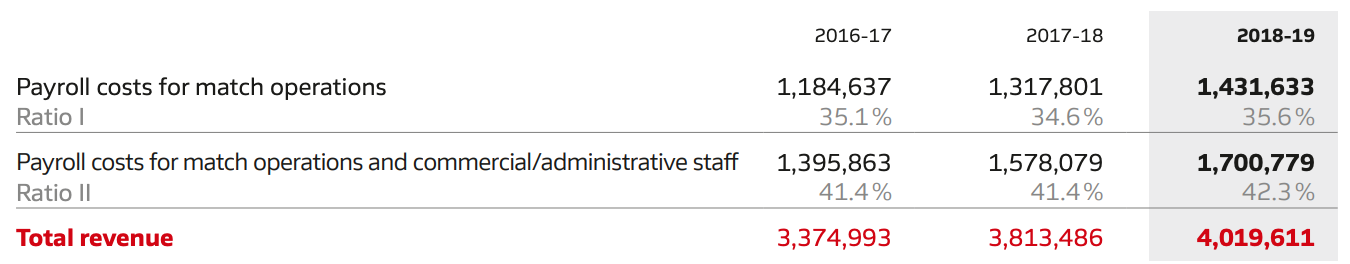
\includegraphics[width=.65\textwidth]{img/wage_germanyA.png} \label{wage_germanyA}} \quad
    \subfloat[][2.Bundesliga]
    {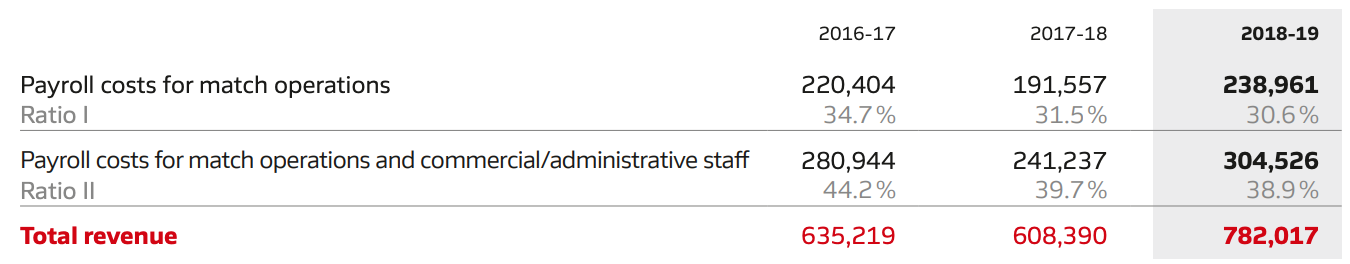
\includegraphics[width=.65\textwidth]{img/wage_germanyB.png} \label{wage_germanyB}}
    \caption{Comparazione stipendi con storico}
    \label{comparazione_stipendi_germania}  
\end{figure}
In Germania \'e radicata sicuramente una cultura legata alla precisione e al rispetto sia delle leggi che delle persone, questo si riflette 
ovviamente in tutti gli ambiti compreso quello del calcio. Come \'e possibile notare, in questo caso, i club prestano molta attenzione a non 
terminare l'anno economico con elevati debiti oppure con risultati ad un passo dal fallimento. Nonostante queste attenzioni, al contrario
di come si potrebbe pensare, arrivano anche risultati dal campo poich\'e negli ultimi anni le squadre tedesche sono sempre riuscite a ritagliarsi 
il proprio spazio nelle competizioni europee, spazio riempito con la vittoria della Champions League da parte del Bayern Monaco nel 2020. 
Rimane sempre per\'o il problema dell'inequit\'a degli stipendi. \'E possibile tuttavia anticipare gi\'a da ora, come in nessuno stato, non si possa
trovare similitudini in termini economici tra i primi due campionati.\newline
Come penultimo campionato oggetto dell'analisi troviamo la \textbf{Spagna}, formato dalla prima divisione \emph{La Liga Santander} e la seconda
\emph{La Liga Smartbank}\footnote{Tutti i dati provengono da: https://www.laliga.com/en-GB/transparency/economic-management/economic-report}.
Il Reddito Complessivo dei due campionati registra una crescita 
dalla stagione 2013/2014. Si parte con un valore combinato di 2.688,5mln€ e si arriva alla stagione 18/19 con un totale di 4.871,4mln€, 
un incremento dell'81,19\%. 
Suddividendo in modo settoriale il Total Income \'e possibile capire come in tutti i vari settori che compongono il Total Income 
si sia verificato un aumento rispetto agli anni precedenti, andando a mostrare quindi come il campionato spagnolo abbia vissuto una forte crescita negli ultimi 6 anni.
I settori sono:
\begin{enumerate}
    \item \textbf{Trasmissioni}: 1665,1 mln€ (+6,2\% rispetto all'anno precedente e +13,6\% in 5 anni). Questa crescita \'e dovuta sopratutto ad una distribuzione 
    centralizzata dei diritti grazie al RDL 5/2015 \footnote{Wikipedia: Real Decreto Ley è un atto avente forza di legge emanato dal Re}.
    \item \textbf{Attivit\'a commerciali}: 983,8 mln€ (+5,5\% rispetto all'anno precedente e +16,7\% in 5 anni). Comprende sponsorizzazioni,
    pubblicit\'a e merchandising.
    \item \textbf{Partite}: 948,6 mln€ (+24,4\% rispetto all'anno precedente e +9,3\% in 5 anni). Comprende le competizioni, biglietti 
    e altre entrate distribuite dalla UEFA.
\end{enumerate}
Il risultato finale del Reddito \'e stato, inoltre, favorito in modo importante dalla crescita di altri 2 fattori che caratterizzano l'attivit\'a tipica del
campionato:
\begin{enumerate}
    \item \textbf{Trasferimenti}: 1006,2 mln€ (+7,2\% rispetto all'anno precedente e +18,1\% in 5 anni).
    \item \textbf{Altre Entrate}: : 267,7 mln€ (+15,7\% rispetto all'anno precedente e -2,8\% in 5 anni). Unico valore che vede una diminuzione
    nel medio periodo ma dovuta al fatto che questa voce, comprendendo accordi di natura finanziaria, assume valori molto diversi nel corso degli anni.
\end{enumerate}
Spostandosi al secondo tema, anche in questo caso come per l'Italia, non viene elaborata un'analisi dettagliata degli stipendi. Nel documento
viene indicato solamente il costo degli stipendi nel corso degli anni e il suo rapporto in percentuale con il Reddito Complessivo e il Fatturato Netto
(figura \ref{wage_spain}).
\begin{figure}
    \centering
    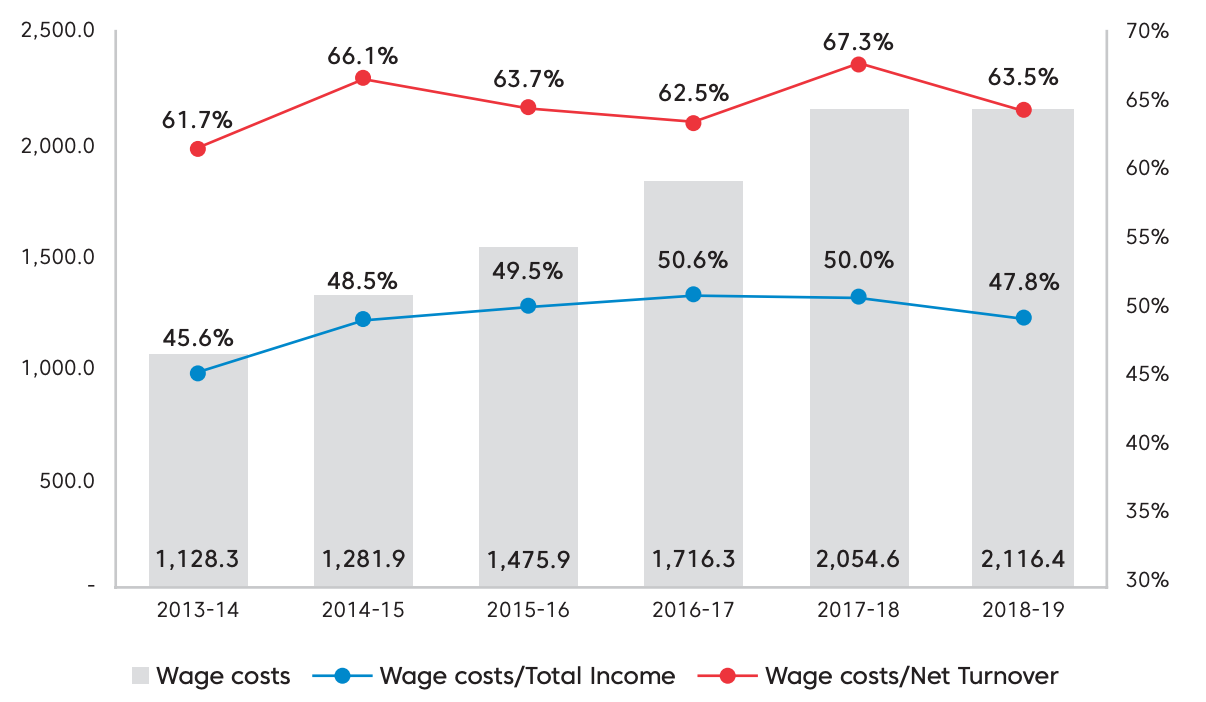
\includegraphics[scale=.5]{img/wage_spain.png}
    \caption{Stipendi La Liga}
    \label{wage_spain}
\end{figure}
La figura mostra come nonostante l'aumento del costo degli stipendi sul totale dei costi, il rapporto con il fatturato vada di anno in anno
a decrescere, mostrando ancora una volta come il campionato spagnolo sia in crescita economica. Un risultato nuovamente positivo \'e stato
sicuramente influenzato dal \emph{\textbf{Salary Cap}} introdotta nel 2013 da parte del CdS\footnote{Wikipedia: Consejo Superior de Deportes cio\'e il massimo organo sportivo a livello nazionale}.
Questa nuova riforma ha il campito di porre dei limiti alle spese dei club riguardo gli stipendi e in generale tutti i costi connessi ai calciatori,
per evitare problematiche presenti ad esempio in Francia dove club con forti disponibilit\'a economiche gareggiano incontrastati nel Paese.\newline
Dovendo fornire un commento/conclusione all'analisi appena svolta \'e possibile affermare come La Liga sia innegabilmente in crescita da 6 
anni a questa parte, essendo il secondo campionato pi\'u visto al mondo con 2.663 mln di spettatori, dietro solo la Premier League a quota 
3.200 mln\footnote{Premier League: https://www.premierleague.com/news/1280062}.\newline
Come ultimo elemento compreso in questa prima analisi suddivisa per Paesi troviamo l'\textbf{Inghilterra}. In questo Paese il calcio 
\'e una vera e propria colonna portante, capace di generare ricavi per 5.440mln£\footnote{https://www2.deloitte.com/global/en/pages/about-deloitte/articles/annual-review-of-football-finance.html}
nella stagione 2017/2018. Il punto di forza \'e sicuramente legato alla vastissima diffusione dei diritti tv che compongono il fattore ricavi
del 59\% ma \'e anche, sopratutto, una questione di lingua dato che l'inglese \'e la lingua pi\'u diffusa in tutto il mondo.\newline
Iniziando a presentare i dati riguardanti l'analisi, la societ\'a Deloitte tramite l'\emph{Annual Review of Football Finance} mostra
l'andamento dei 5 maggiori campionati europei e si sofferma inoltre su quello inglese. Questo report mostra come in solo 3 anni i \textbf{ricavi} 
dei club di \emph{Premier League}, il primo campionato inglese, siano aumentati del 41,71\% passando da 3.639mln£ a 5.157mln£ valori a cui solo
la Bundesliga riesce quantomeno ad avvicinarcisi. Il punto di forza, come gi\'a affermato prima, \'e sicuramente i ricavi generati dai diritti
tv che compongono ogni anni pi\'u della met\'a dei ricavi totali; anche la parte denominata \emph{Commercial} non \'e da meno, con valori
che si aggirano sempre intorno ai 1.500mln£. Il vero problema per\'o si presenta se si va a confrontare i ricavi dei cosiddetti \emph{Big Six}, 
i 6 club che hanno fatto la storia del campionato: Arsenal, Manchester City, Manchester United, Tottenham, Chelsea e Liverpool con i ricavi
generati dalle altre societ\'a.
\begin{figure}
    \centering
    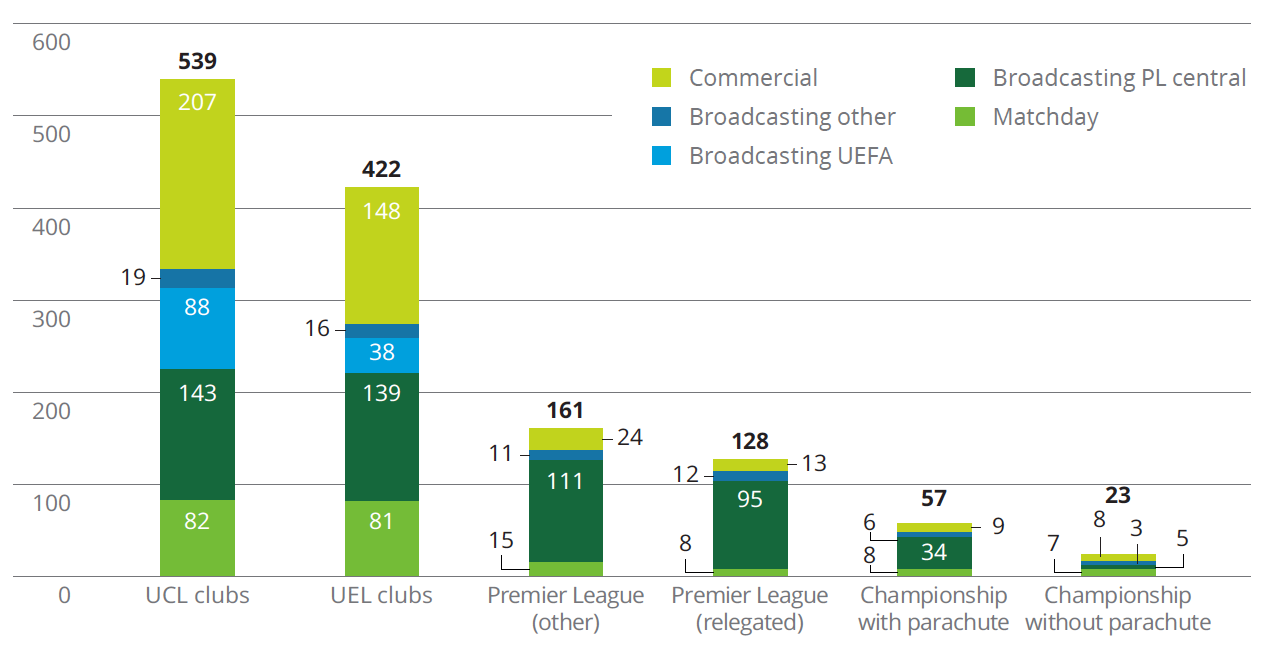
\includegraphics[scale=0.5]{img/ricavi_premier.png}
    \caption{Confronto ricavi dei club di Premier League divisi per gruppi}
    \label{ricavi_premier}
\end{figure} 
La figuta \ref{ricavi_premier} permette di visualizzare immediatamente questa differenza. L'ultima classificata tra i \emph{Big Six},
l'Arsenal ha generato ricavi 393mln£ mentre il West Ham, classificatosi settimo e quindi una posizione immediatamente sotto l'Arsenal, ha 
prodotto per 193mln£, una differenza di ricavi di 200mln£ con una sola posizione in classifica di distacco. Nel grafico sono inoltre riportati
i club retrocessi "con paracadute", un sistema che tramite i diritti di trasmissione aiuta economicamente i club nelle posizioni
pi\'u basse della classifica.\newline
Sempre all'intrerno dell'analisi prodotta da Deloitte \'e contenuto un approfondimento sugli \textbf{stipendi}. Anche in questo caso, se a
primo impatto i dati non sembrano preoccupare, se si analizzano a fondo si pu\'o notare come gi\'a dalla stagione 2018/2019 ci fossero segni
di preoccupazione. Il peso degli stipendi per i club della Premier League in quella stagione ammontava a 3.155mln£, il 61\% dei ricavi contro il 
59\% dell'anno precedente. Questo aumento ha fatto si che si presentassero alla fine dell'esercizio ben 6 club con una perdita operativa, il 
peggior risultato dal 2012/2013.\newline
\section{Analisi per Club}
La seconda parte di questa trattazione andr\'a a prendere in esame i club pi\'u importanti oppure quelli che saranno pi\'u utili al fine 
delle successive analisi dei diversi Paesi elencati nel sottocapitolo precedente. Per quanto riguarda l'Italia verr\'a analizzata la \textbf{Juventus},
per la Francia il \textbf{Paris Saint Germain}, per la Germania il \textbf{Borussia Dortmund}, per la Spagna il \textbf{Barcellona} e infine per l'Inghilterra il 
\textbf{Manchester City}.\newline
L'analisi verr\'a svolta considerando 4 macro-categorie:
\begin{enumerate}
    \item Analisi dei Ricavi: similmente a come fatto prima ma in modo pi\'u specifico, in questa parte verr\'a fatta un'analisi relativa
        ai diversi tipi di ricavo e la loro incidenza rispetto ai ricavi totali; 
    \item Analisi della Liquidit\'a: in questa sezione verranno analizzate le voci di bilancio relative agli impegni delle societ\'a
        nel breve/medio periodo;
    \item Analisi della Solidit\'a: qu\'i invece verranno prese in analisi le capacit\'a dei club di far fronte ad impegni su un periodo di
        tempo pi\'u lungo, evidenziando o meno il peso dei mezzi propri e la dipendenza dai finanziatori terzi;
    \item Analisi della Redditivit\'a: nella penultima categoria di analisi viene "tagliato" in modo orizzontale il bilancio, andando quindi
        a considerare sia voci di Stato Patrimoniale sia voci di Conto Economico per capire gli investimenti effettuati e i risultati ottenuti;
\end{enumerate} 
\subsection{Juventus}
Il primo club ad essere analizzato \'e appunto la Juventus, uno dei club pi\'u famosi e vincenti in Italia e tredicesima per numero di tifosi 
in tutto il mondo. Il potere \'e sempre stato in mano alla famiglia Agnelli, che a partire dal 1923 ha guidato il club torinese ad un lungo
\emph{palmares} di successi\footnote{https://it.wikipedia.org/wiki/Storia\_della\_Juventus\_Football\_Club}. Alla stagione 2018/2019 vantava: 34 Scudetti di cui dal 2012 sette conquistati consecutivamente, 13
Coppe Italia, 7 Supercoppe Italiane, 2 Champions League e 2 Coppe Intercontinentali.\newline
\begin{enumerate}
    \item Analisi dei Ricavi:\newline
        Per questa primo punto \'e necessario prendere in considerazione il prospetto di Conto Economico al 30 Giugno 2019.
        Verrano messi in relazione alcune voce della sezione ricavi del CE con il totale dei ricavi generati sottraendo per\'o la voce
        "Altri Ricavi" in modo da prendere in considerazione solo le voci pi\'u rilevanti.
        \begin{figure}
            \centering
            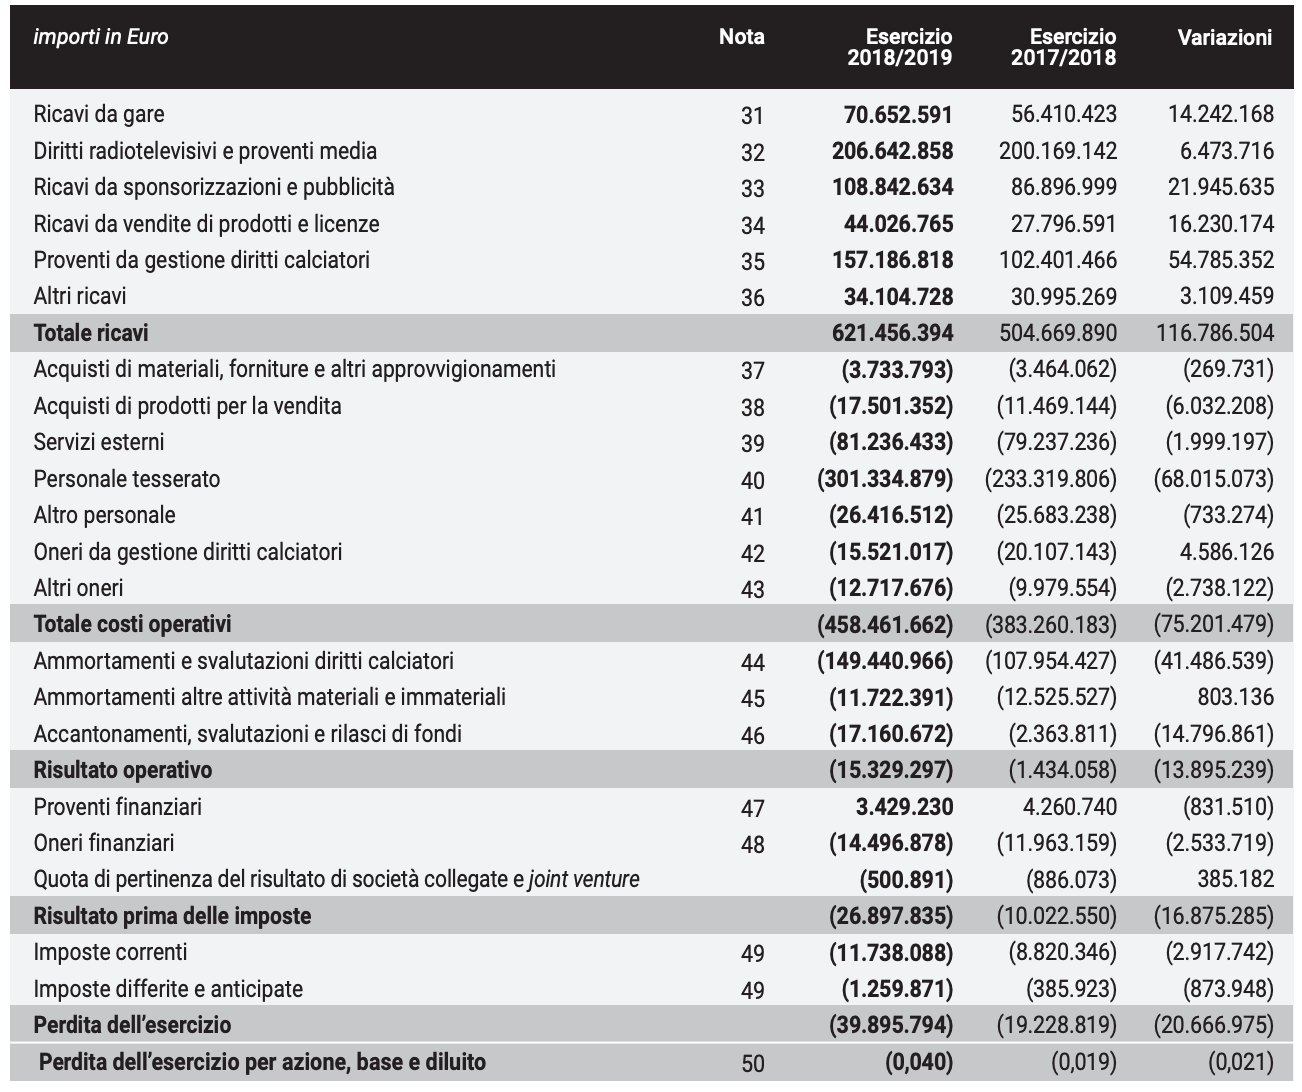
\includegraphics[scale=.4]{img/CE_juve.png}
            \caption{Conto Economico Juventus al 30 Giugno 2019}
            \label{ce_juve}
        \end{figure}\newline
        \begin{equation}
            \frac{\text{Ricavi da gare}}{\text{Totale Ricavi}} = \frac{70.652.591}{587.351.666} = \mathbf{12,02\%}
            \label{eqn: gare_juve}
        \end{equation}
        \begin{equation}
            \frac{\text{Diritti TV}}{\text{Totale Ricavi}} = \frac{206.642.858}{587.351.666} = \mathbf{35,18\%}
            \label{eqn: tv_juve}
        \end{equation}
        \begin{equation}
            \frac{\text{Ricavi commerciali}}{\text{Totale Ricavi}} = \frac{152.869.399}{587.351.666} = \mathbf{26,02\%}
            \label{eqn: commerc_juve}
        \end{equation}
        Per quanto la Juventus sia tra le poche societ\'a nel panorama italiano ad avere uno stadio di propriet\'a, 
        insieme a Udinese e Sassuolo, il profilo dei suoi ricavi non \'e minimamente paragonabile alle concorrenti Europee.
        Come si vedrà pi\'u avanti con l’analisi dei bilanci di squadre come Barcellona e Manchester City, sopratutto la voce dei Ricavi
        da Stadio e Ricavi Commerciali non \'e minimamente confrontabile. Un secondo problema che deve far allarmare la societ\'a Piemontese
        \'e il fatto che i ricavi da gare siano molto bassi a causa di una inspiegabile bassa affluenza di tifosi alla stadio. Basti pensare 
        che l'Allianz Stadium ha una media spettatori simile a quella dell'Artemio Franchi di Firenze, palcoscenico piuttosto differente da 
        quello di Torino\footnote{TransferMarket: https://www.transfermarkt.it/ac-florenz/besucherzahlenentwicklung/verein/430}.
    \item Analisi della liquidit\'a:\newline
        Per questo punto andranno invece a considerarsi le voci presenti nello Stato Patrimoniale del Bilancio d'Esercizio.
        \begin{figure}
            \centering
            \subfloat[][Stato Patrimoniale attivo al 30 Giugno 2019]
            {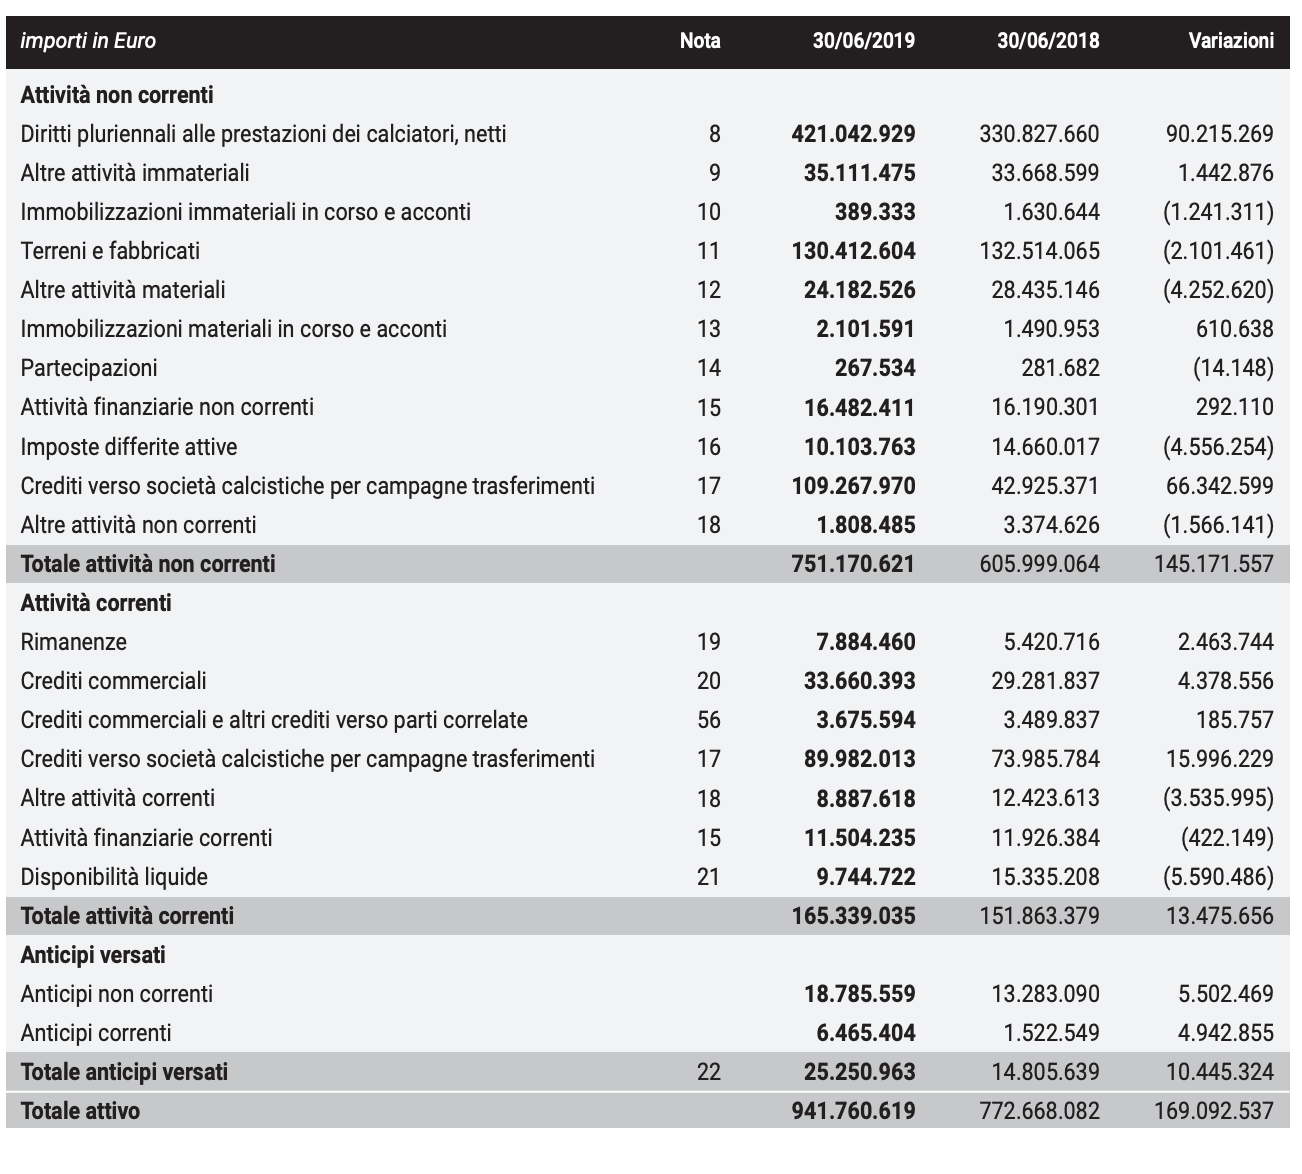
\includegraphics[width=.45\textwidth]{img/SP_attivo_juve.png} \label{sp_attivo_juve}} \quad
            \subfloat[][Stato Patrimoniale passivo al 30 Giugno 2019]
            {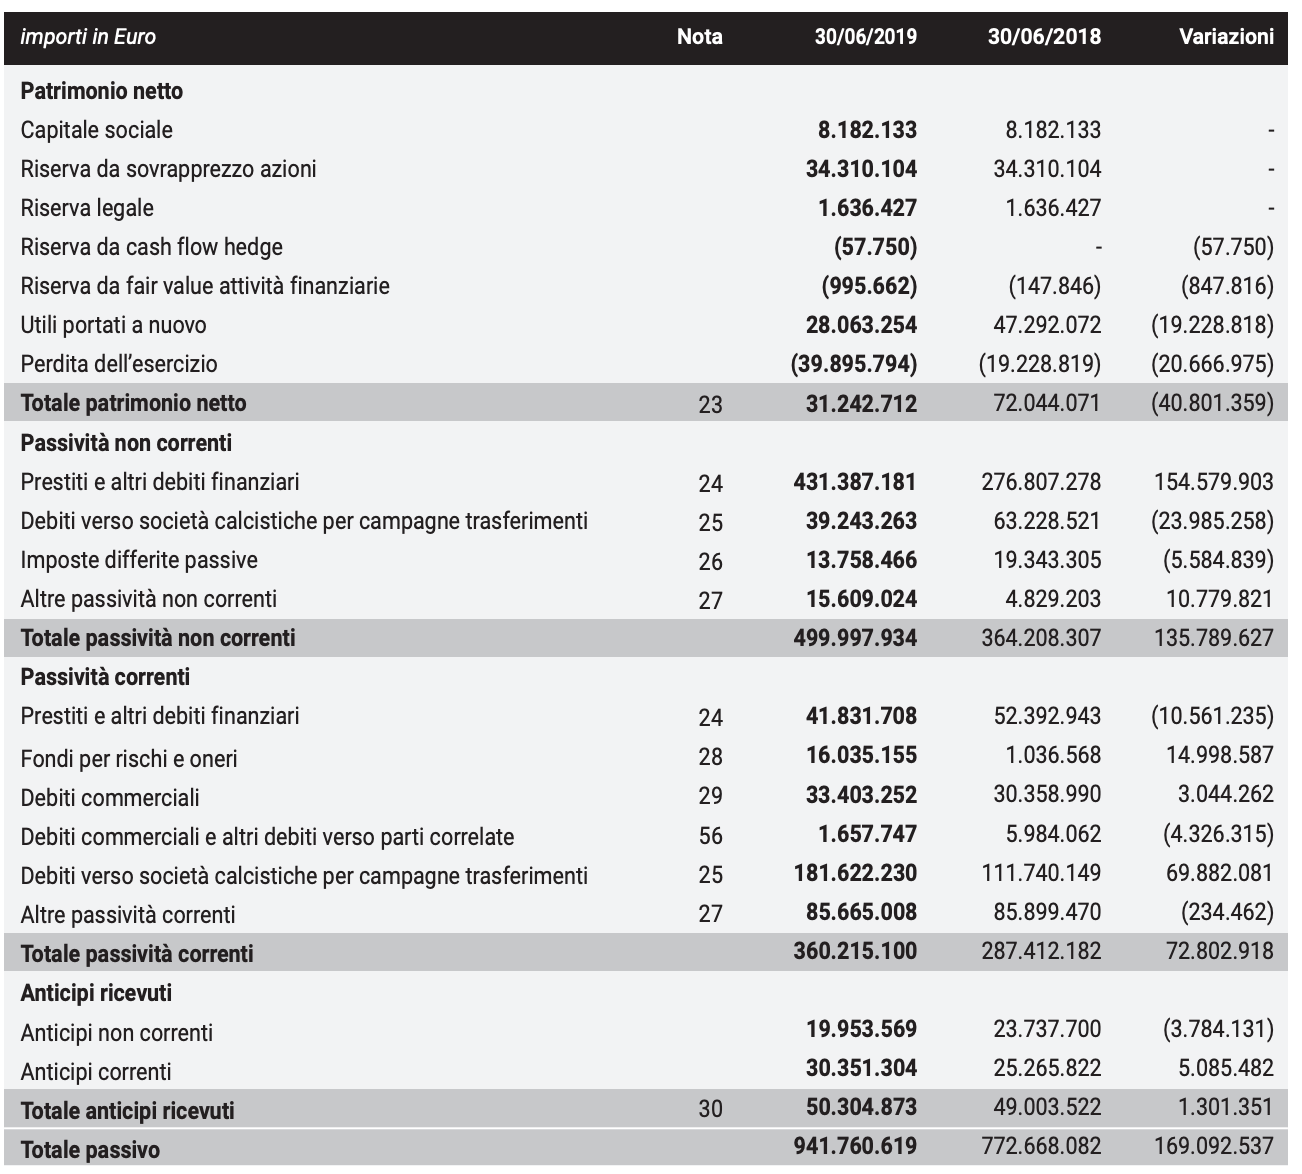
\includegraphics[width=.45\textwidth]{img/SP_passivo_juve.png} \label{sp_passivo_juve}}
            \caption{Stato Patrimoniale Juventus al 30 Giungno 2019}
            \label{sp_juve}  
        \end{figure}
        \begin{equation}
                \text{Margine di Tesoreria} = 157.454.575-390.566.404 = \mathbf{-233.111.829\mbox{\euro}}
            \label{eqn: marg_teso_juve}
        \end{equation}
        \begin{equation}
                \text{Indice di liquidit\'a primaria} = \frac{157.454.575}{390.566.404} = \mathbf{40,31\%}
            \label{eqn: ind_liq_juve}
        \end{equation}
        Per quanto riguarda l'analisi degli indici di Stato Patrimoniale che identificano quanto una societ\'a \'e in grado di far 
        fronte, con mezzi correnti e non correnti, alle passivit\'a a breve termine la situazione della Juventus non \'e del tutto positiva.
        Per essere considerato efficace il Margine di Tesoreria e il relativo Indice di Liquidit\'a primaria devono essere entrambi positivi
        e maggiori di uno\footnote{Valter Cantino, Paola De Bernardi, Alain Devalle (2018) Sistemi di rilevazione e misurazione delle performance aziendali Torino: G. Giappichelli};
        in entrambi i casi questi requisiti non vengono soddisfatti. I dati peggiorano anche rispetto all'anno precedente
        questo a causa dell'acquisto del calciatore Cristiano Ronaldo, il quale in Bilancio ha il suo peso con un 
        prezzo di acquisto di 115mln€ e uno stipendio lordo di 57mln€. Questo problema per\'o \'e risaputo: tutti i club del mondo si indebitano,
        sopratutto nei confronti dei calciatori che con il passare degli anni avanzano richieste sempre maggiori e, per far fronte a queste 
        richieste i club creano altro debito, andando a creare un vero e proprio circolo vizioso.
    \item Analisi della solidit\'a:\newline
        \begin{equation}
            \text{Grado di Indpendenza Finanziaria} = \frac{31.242.712}{941.760.619} = \mathbf{3,31\%}
        \label{eqn: indeb_juve}
        \end{equation}
        \begin{equation}
            \text{Margine di Struttura} = 31.242.712-613.240.458 = \mathbf{-581.997.746\mbox{\euro}}
            \label{eqn: marg_strutt_juve}
        \end{equation}
        In questa sezione la Juventus presenta due situazioni nuovamente negative: a causa del risultato in rosso dell'anno
        precedente il Patrimonio Netto \'e diminuito e di conseguenza il grado di indipendenza finanziaria si attesta al 3,31\%,
        un valore che mostra la dipendenza della societ\'a da mezzi esterni; il Margine di Struttura
        visualizza invece la capacit\'a dei mezzi propri di coprire le immobilizzazioni e capire se serve ricorrere a mezzi terzi. Anche in questo 
        caso un valore negativo \'e preoccupante perch\'e sta a significare che per quasi 600mln€ serviranno mezzi terzi.\newpage
    \item Analisi della Redditivit\'a:\newline
        \begin{equation}
            \text{ROI} = \frac{-15.329.297}{941.760.619} = \mathbf{-1,6\%}
        \label{eqn: roi_juve}
        \end{equation}
        \begin{equation}
            \text{ROE} = \frac{-39.895.794}{31.242.712} = \mathbf{-127,69\%}
        \label{eqn: roe_juve}
        \end{equation}
        Questo ultimo punto dell'analisi evidenzia in modo immediato come la societ\'a stia rischiando molto in campo economico: troviamo in 
        primo luogo un peggioramento significativo del Reddito Operativo che passa da -1.434.058€ nel 2017 a -15.239.297€ nel 2018 (una variazione del 962\%);
        anche la perdita d'esercizio ha un andmento simile con uno scostamento di 20mln€ rispetto all'anno precedente. Questo peggioramento
        cos\'i importante dei valori \'e dovuto sopratutto all'aumento del personale tesserato e alla voce "Ammortamenti e svalutazione diritti calciatori",
        sempre legata all'acquisto di Cristiano Ronaldo.
\end{enumerate}
\subsection{Paris Saint Germain}
Spostandosi in Francia troviamo il Paris Saint Germain, squadra famosa in tutto il mondo grazie alla potenza economica dello sceicco Nasser Al-Khelaïfi 
che, nel 2011\footnote{Wikipedia: https://it.wikipedia.org/wiki/Nasser\_Al-Khela\%C3\%AFfi}, acquista la maggioranza delle quote della societ\'a e da il via 
ad un periodo di spese folli per creare un vero e proprio impero.
Queste cifre spese non sono per\'o servite ad ottenere risultati significativi, l'unico traguardo degno di nota della squadra dal 2011 ad oggi
\'e stata la finale di Champions League nel 2020, persa con il Bayern Monaco.\newpage
\begin{enumerate}
    \item Analisi dei Ricavi:\newline
        \begin{figure}
            \centering
            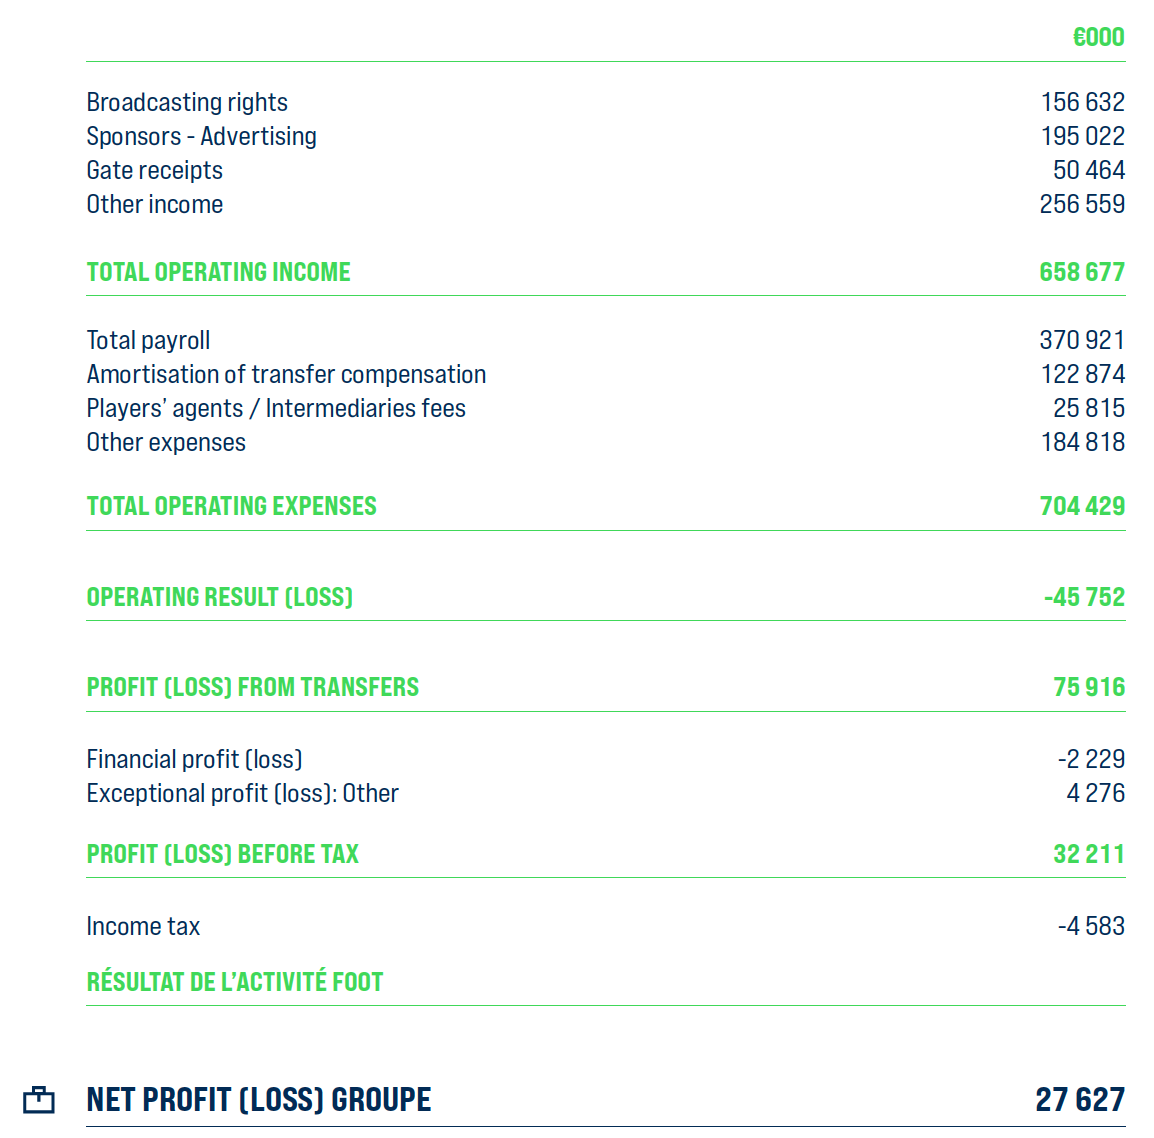
\includegraphics[scale=.4]{img/CE_psg.png}
            \caption{Conto Economico Paris Saint Germain al 30 Giugno 2019}
            \label{ce_psg}
        \end{figure}\newline
        \begin{equation}
            \frac{\text{Ricavi da gare}}{\text{Totale Ricavi}} = \frac{50.464.000}{658.677.000} = \mathbf{7,68\%}
            \label{eqn: gare_psg}
        \end{equation}
        \begin{equation}
            \frac{\text{Diritti TV}}{\text{Totale Ricavi}} = \frac{156.632.000}{658.677.000} = \mathbf{23,77\%}
            \label{eqn: tv_psg}
        \end{equation}
        \begin{equation}
            \frac{\text{Ricavi commerciali}}{\text{Totale Ricavi}} = \frac{195.022.000}{658.677.000} = \mathbf{29,60\%}
            \label{eqn: commerc_psg}
        \end{equation}
        In questo scenario troviamo una situazione abbastanza differente. Sebbene il Paris Saint Germain sia molto seguita in Europa e nel
        mondo i ricavi da gare e diritti Tv sono inferiori (rapportati al Totale Incassi) rispetto a quelli della Juventus\footnote{https://www.lfp.fr/dncg/rapports}: questo perch\'e
        in Francia non troviamo una cos\'i radicata cultura calcistica, sopratutto per quanto riguarda i singoli club e, mancando di \emph{appeal}
        internazionale, il campionato francese non pu\'o contare molto sulla vendita della trasmissione delle partite. I Ricavi Commerciali invece
        sono leggermente superiori per il motivo appunto che data la grande importanza a livello mondiale del club, esso vende maggiormente in tutto il mondo.
    \item Analisi della liquidit\'a:\newline
        \begin{figure}
            \centering
            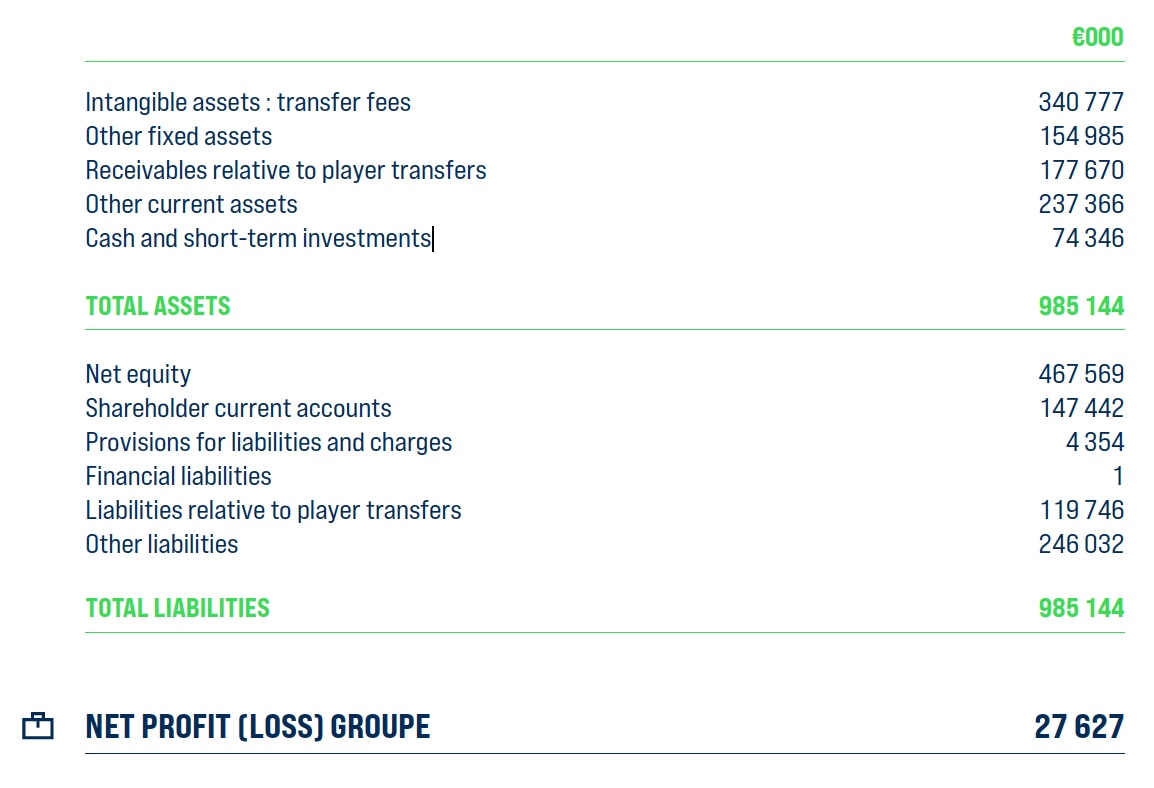
\includegraphics[scale=.5]{img/SP_psg.png}
            \caption{Stato Patrimoniale Paris Saint Germain al 30 Giungno 2019}
            \label{sp_psg}  
        \end{figure}
        \begin{equation}
                \text{Margine di Tesoreria} = 74.346.000-246.032.000 = \mathbf{-171.786.000\mbox{\euro}}
            \label{eqn: marg_teso_psg}
        \end{equation}
        \begin{equation}
                \text{Indice di liquidit\'a primaria} = \frac{74.346.000}{246.032.000} = \mathbf{30,21\%}
            \label{eqn: ind_liq_psg}
        \end{equation}
       Anche in questo caso non si presenta una situazione positiva: l'equazione \ref{eqn: marg_teso_psg} mostra come anche in questo caso il 
       risultato sia negativo, anche se in valore minore. Questo probabilmente perch\'e il PSG possedendo una quantit\'a elevatissima di risorse
       liquide e immediate, riesce comunque a tenere sotto controllo le passivit\'a a breve termine.
    \item Analisi della solidit\'a:\newline
        \begin{equation}
            \text{Grado di Indipendenza finanziaria} = \frac{467.569.000}{985.144.000} = \mathbf{47,46\%}
        \label{eqn: indeb_psg}
        \end{equation}
        \begin{equation}
            \text{Margine di Struttura} = 467.569.000-495.762.000 = \mathbf{-28.193.000\mbox{\euro}}
            \label{eqn: marg_strutt_psg}
        \end{equation}
        Contrariamente a quanto si \'e visto per la Juventus, la squadra di Parigi \'e maggiormente in grado di affrontare
        debiti e passivit\'a finanziarie tramite il capitale proprio, questo accade sicuramente grazie alla forte capitalizzazione
        che apporta il presidente. Tramite il margine di struttura, invece, possiamo capire come anche in questo caso, con solo mezzi propri non si riesca a coprire il valore
        delle immobilizzazioni anche se, 28mln€ di differenza non sono cos\'i elevati considerando i numeri di oggi.
    \item Analisi della Redditivit\'a:\newline
        \begin{equation}
            \text{ROI} = \frac{-45.752.000}{985.144.000} = \mathbf{-4,6\%}
        \label{eqn: roi_psg}
        \end{equation}
        \begin{equation}
            \text{ROE} = \frac{27.627.000}{467.569.000} = \mathbf{5,90\%}
        \label{eqn: roe_psg}
        \end{equation}
        Questo ultimo punto dell'analisi mette in mostra due risultati molto differenti: da una parte troviamo un ROI negativo dovuto ad
        un risultato netto negativo a causa della grande spesa per gli stipendi (370.921.000€) ed un Capitale Investito anch'esso molto elevato;
        dall'altro lato invece il ROE assume un valore positivo, anche se non ancora considerabile buono, grazie al profitto generato dalla 
        vendita dei giocatori e dalla non elevata tassazione applicata in Francia
\end{enumerate}
\subsection{Borussia Dortmund}
Continuando la disamina dei vari club Europei, ora \'e il momento del Borussia Dortmund. Il club tedesco anche se spesso oscurato dai continui
successi del Bayern Monaco è comunque riuscito a ritagliarsi il suo spazio in patria e in Europa, conquistando: 8 campionati tedeschi, 5 supercoppe di Germania, 4 coppe nazionali, 1 Champions League e 1 Coppa
intercontinentale\footnote{https://it.wikipedia.org/wiki/Ballspielverein\_Borussia\_09\_Dortmund}. 
\begin{enumerate}
    \item Analisi dei Ricavi:\newline
        \begin{figure}
            \centering
            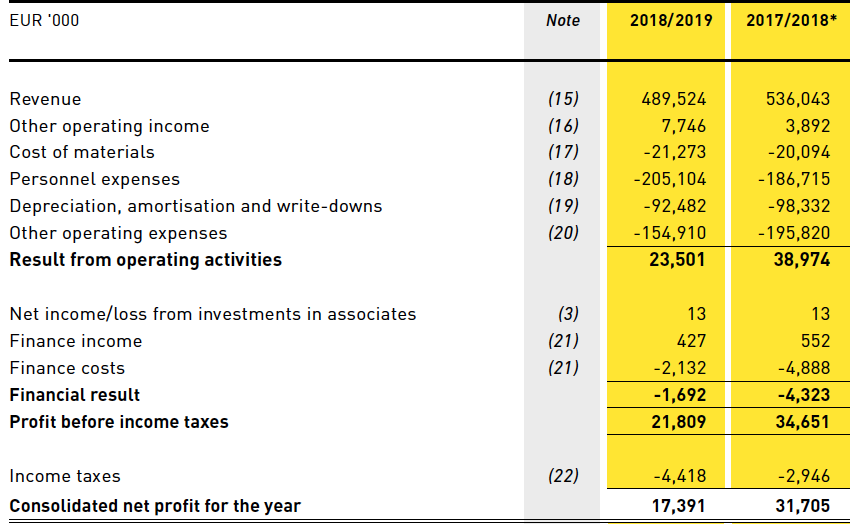
\includegraphics[scale=.4]{img/CE_dor.png}
            \caption{Conto Economico Borussia Dortmund al 30 Giugno 2019}
            \label{ce_dor}
        \end{figure}\newline
        \begin{equation}
            \frac{\text{Ricavi da gare}}{\text{Totale Ricavi}} = \frac{44.659.000}{498.777.000} = \mathbf{8,95\%}
            \label{eqn: gare_dor}
        \end{equation}
        \begin{equation}
            \frac{\text{Diritti TV}}{\text{Totale Ricavi}} = \frac{167.349.000}{498.777.000} = \mathbf{33,55\%}
            \label{eqn: tv_dor}
        \end{equation}
        \begin{equation}
            \frac{\text{Ricavi commerciali}}{\text{Totale Ricavi}} = \frac{130.002.000}{498.777.000} = \mathbf{26,06\%}
            \label{eqn: commerc_dor}
        \end{equation}
        In Germania la situazione \'e abbastanza analoga come per l'Italia: i ricavi da gare sono pi\'u bassi ma salgono rispetto all'anno precedente,
        i ricavi da diritti tv rimangono sulla stessa linea ma scendono di qualche punto percentuale anche i ricavi commerciali, probabilmente
        per il fatto che il Borussia non \'e cos\'i largamente conosciuto nel mondo come pu\'o esserlo la Juventus.
    \item Analisi della liquidit\'a:\newline
        \begin{figure}
            \centering
            \subfloat[][Stato Patrimoniale attivo al 30 Giugno 2019]
            {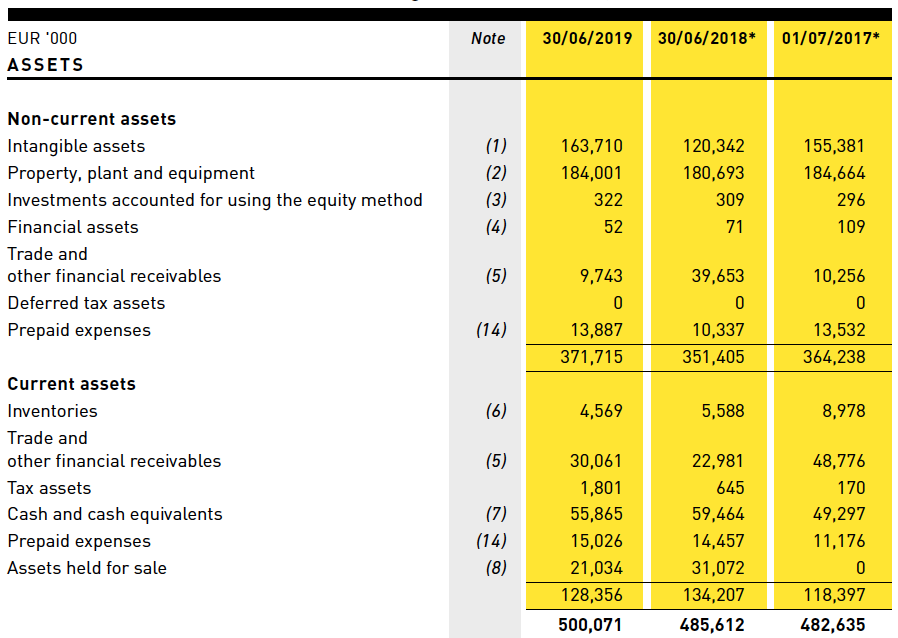
\includegraphics[width=.45\textwidth]{img/SP_attivo_dor.png} \label{sp_attivo_dor}} \quad
            \subfloat[][Stato Patrimoniale passivo al 30 Giugno 2019]
            {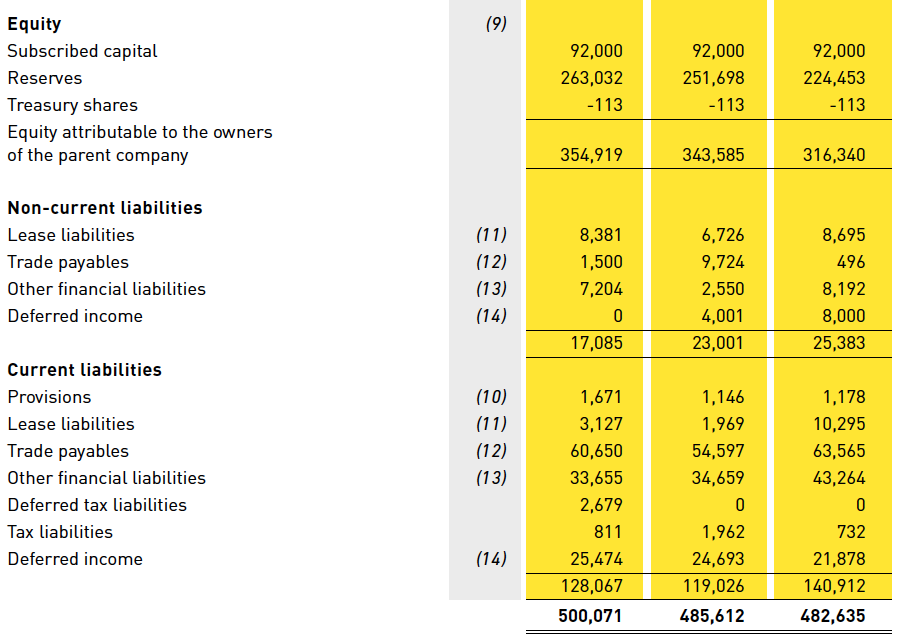
\includegraphics[width=.45\textwidth]{img/SP_passivo_dor.png} \label{sp_passivo_dor}}
            \caption{Stato Patrimoniale Borussia Dortmund al 30 Giungno 2019}
            \label{sp_dor}  
        \end{figure}
        \begin{equation}
                \text{Margine di Tesoreria} = 123.787.000-128.067.000 = \mathbf{-4.280.000\mbox{\euro}}
            \label{eqn: marg_teso_dor}
        \end{equation}
        \begin{equation}
                \text{Indice di liquidit\'a primaria} = \frac{123.787.000}{128.067.000} = \mathbf{96,65\%}
            \label{eqn: ind_liq_dor}
        \end{equation}
       Per la prima volta troviamo una situazione positiva per la posizione di liquidit\'a: il margine di tesoreria \'e si negativo, ma di solo
       4mln€ e l'indice di liquidit\'a spiega come le passivit\'a a breve siano coperte per il 96\% da mezzi liquidi e quindi subito disponbili,
       rendendo il Borussia una societ\'a che nel complesso puo\'o far fronte completamente ai debiti nel breve termine.
    \item Analisi della solidit\'a:\newline
        \begin{equation}
            \text{Grado di Indipendenza Finanziaria} = \frac{354.919.000}{500.071.000} = \mathbf{70,97\%}
        \label{eqn: indeb_dor}
        \end{equation}
        \begin{equation}
            \text{Margine di Struttura} = 354.919.000-348.085.000 = \mathbf{6.834.000\mbox{\euro}}
            \label{eqn: marg_strutt_dor}
        \end{equation}
        Anche in questo caso troviamo una situazione molto positiva: il grado di indipendenza finanziaria mostra che tramite il patrimonio
        netto la societ\'a riesce ad affrontare il 70\% del valore delle passivit\'a, a riprova della oculata gestione economica tedesca.
        Anche il margine di struttura non \'e da meno dato che per la prima volta troviamo un valore positivo, a dimostrazione tramite i mezzi
        propri sono pefettamente in grado di far fronte a tutte immobilizzazioni.  \newline
    \item Analisi della Redditivit\'a:\newline
        \begin{equation}
            \text{ROI} = \frac{23.501.000}{500.071.000} = \mathbf{4,6\%}
        \label{eqn: roi_dor}
        \end{equation}
        \begin{equation}
            \text{ROE} = \frac{17.391.000}{354.919.000} = \mathbf{4,8\%}
        \label{eqn: roe_dor}
        \end{equation}
        Anche in quest'ultimo caso i risultati sono incoraggianti: il ROI \'e positivo grazie ovviamente al fatto che \'e presente un 
        risultato d'esercizio positivo (anche se in diminuzione rispetto all'anno precedente) e con un valore di 4,6\% evidenzia la capacit\'a
        della societ\'a di far fruttare gli investimenti effettuati; il ROE, anch'esso positivo evidenzia invece come gli investimenti fatti con 
        capitale proprio stia andando nella giusta direzione.
\end{enumerate}
\subsection{Barcellona}
Quarto club soggetto dell'analisi \'e il Barcellona, una delle squadre pi\'u titolate e tifate al mondo la quale vanta un \emph{palmares} di:
26 campionati, 31 Coppe di Spagna, 2 Coppe della Liga, 13 Supercoppe di Spagna e 3 Coppe de Oro Argentina\footnote{https://it.wikipedia.org/wiki/Futbol\_Club\_Barcelona}.
\'E l'unica squadra, insieme al Bayern Monaco, ad aver conquistato il \emph{sextuple} riuscendo a vincere tutte le 6 competizioni nazionali e
internazionali disponibili durante l'anno. Insieme al Real Madrid formano una delle rivalit\'a pi\'u antiche e accese della storia Europea, 
possedendo anche un nome unico per la partita con quest'ultima: \emph{El Clasico}.\newpage
\begin{enumerate}
    \item Analisi dei Ricavi:\newline
        \begin{figure}
            \centering
            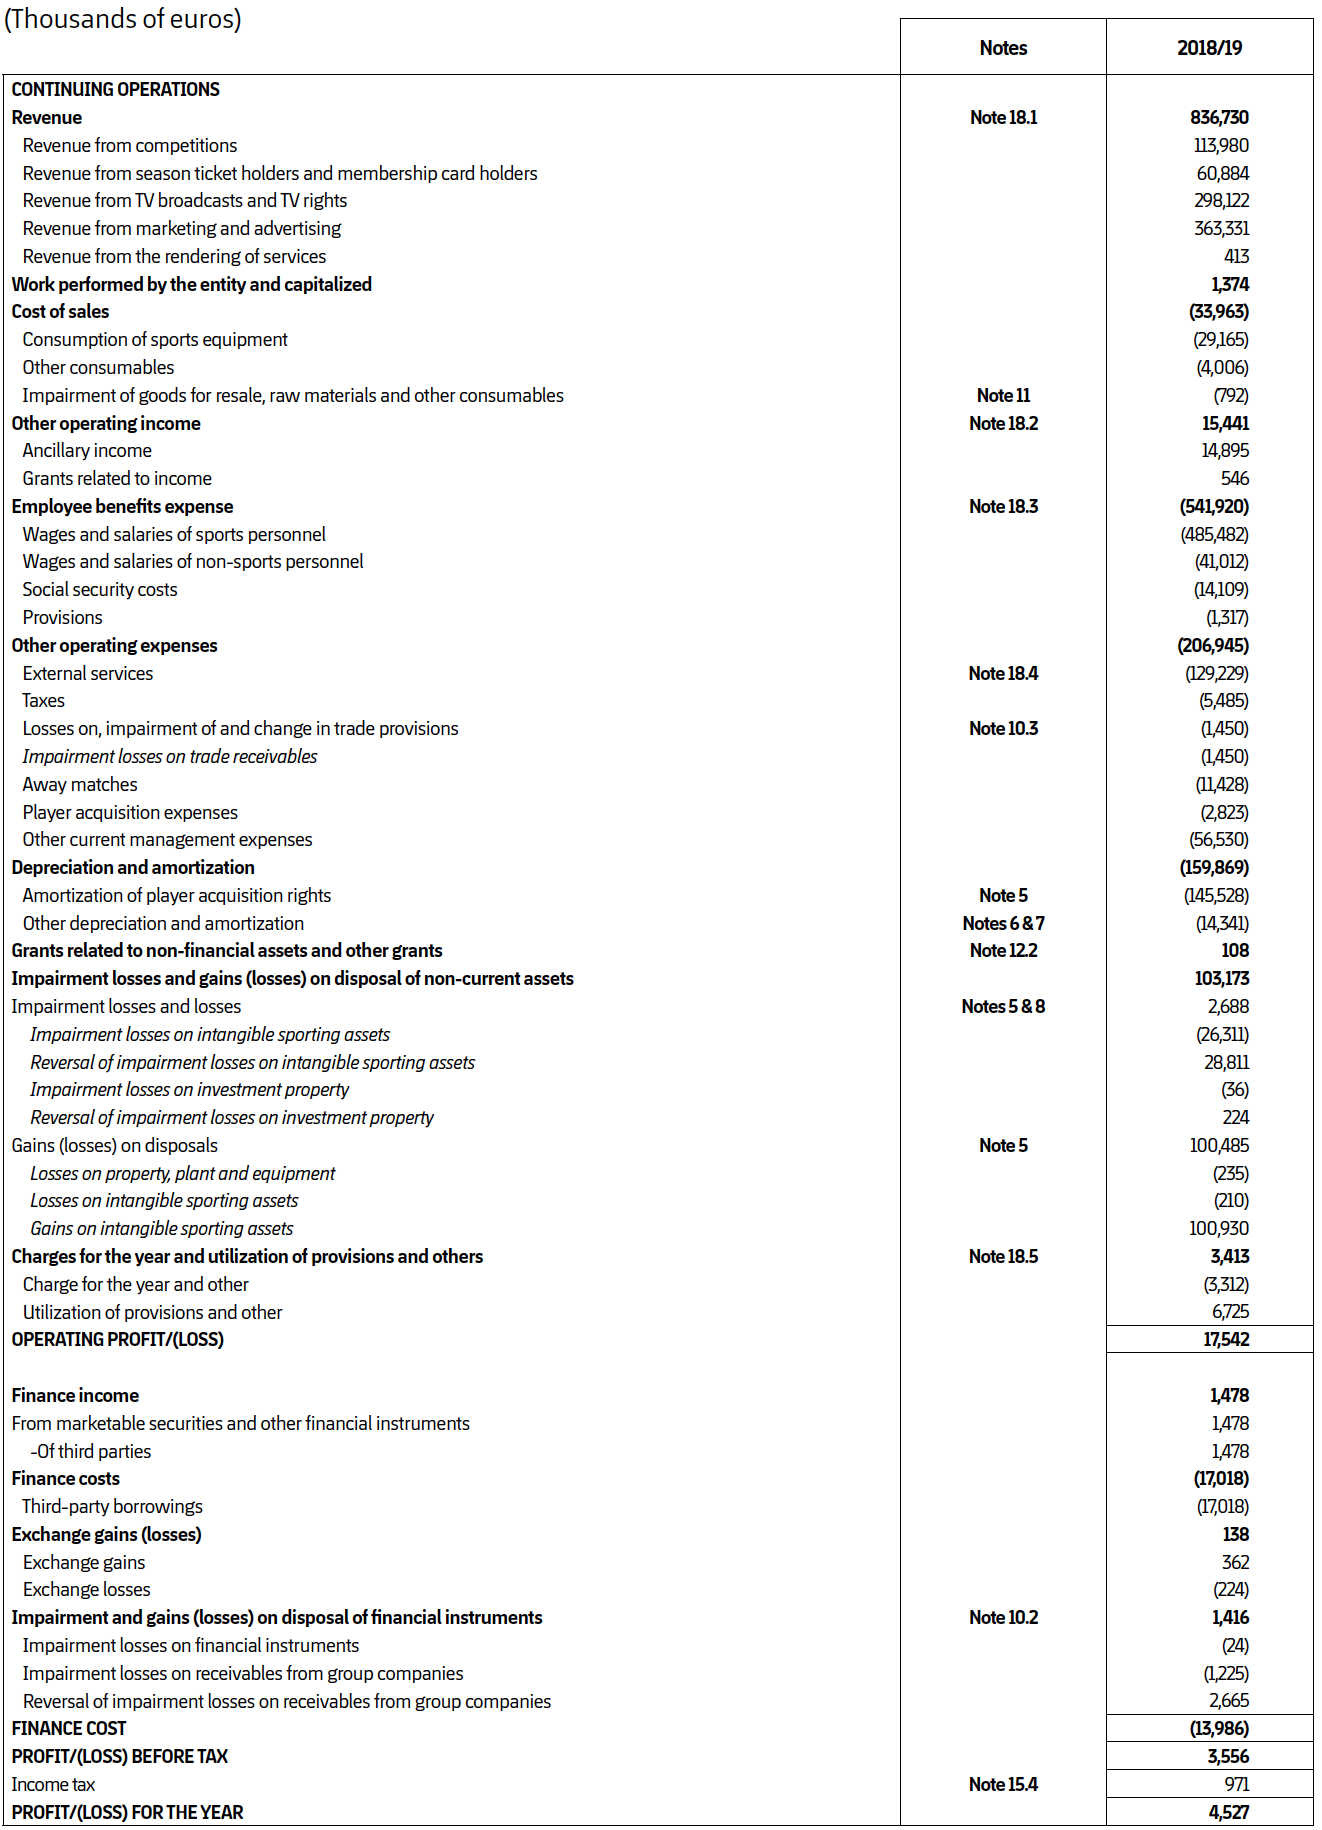
\includegraphics[scale=.5]{img/CE_barca.png}
            \caption{Conto Economico Barcellona al 30 Giugno 2019}
            \label{ce_barca}
        \end{figure}\newline
        \begin{equation}
            \frac{\text{Ricavi da gare}}{\text{Totale Ricavi}} = \frac{170.864.000}{837.730.000} = \mathbf{20,8\%}
            \label{eqn: gare_barca}
        \end{equation}
        \begin{equation}
            \frac{\text{Diritti TV}}{\text{Totale Ricavi}} = \frac{298.122.000}{837.730.000} = \mathbf{35,62\%}
            \label{eqn: tv_barca}
        \end{equation}
        \begin{equation}
            \frac{\text{Ricavi commerciali}}{\text{Totale Ricavi}} = \frac{363.331.000}{837.730.000} = \mathbf{43,42\%}
            \label{eqn: commerc_barca}
        \end{equation}
        La premessa fatta poco prima si riconferma in questa sezione: la parte dei ricavi commerciali copre quasi la met\'a dei ricavi totale,
        a riprova di quanto sia famosa la societ\'a in tutto il mondo; anche i diritti tv prendono una bella fetta del totale dato che
        la Liga Santander \'e molto seguita in tutta Europa ma anche in altri paesi di lingua Spagnola; i ricavi da gare hanno anch'essi 
        una discreta importanza a dimostrazione di come il calcio in Spagna sia molto seguito.
    \item Analisi della liquidit\'a:\newline
        \begin{figure}
            \centering
            \subfloat[][Stato Patrimoniale attivo al 30 Giugno 2019]
            {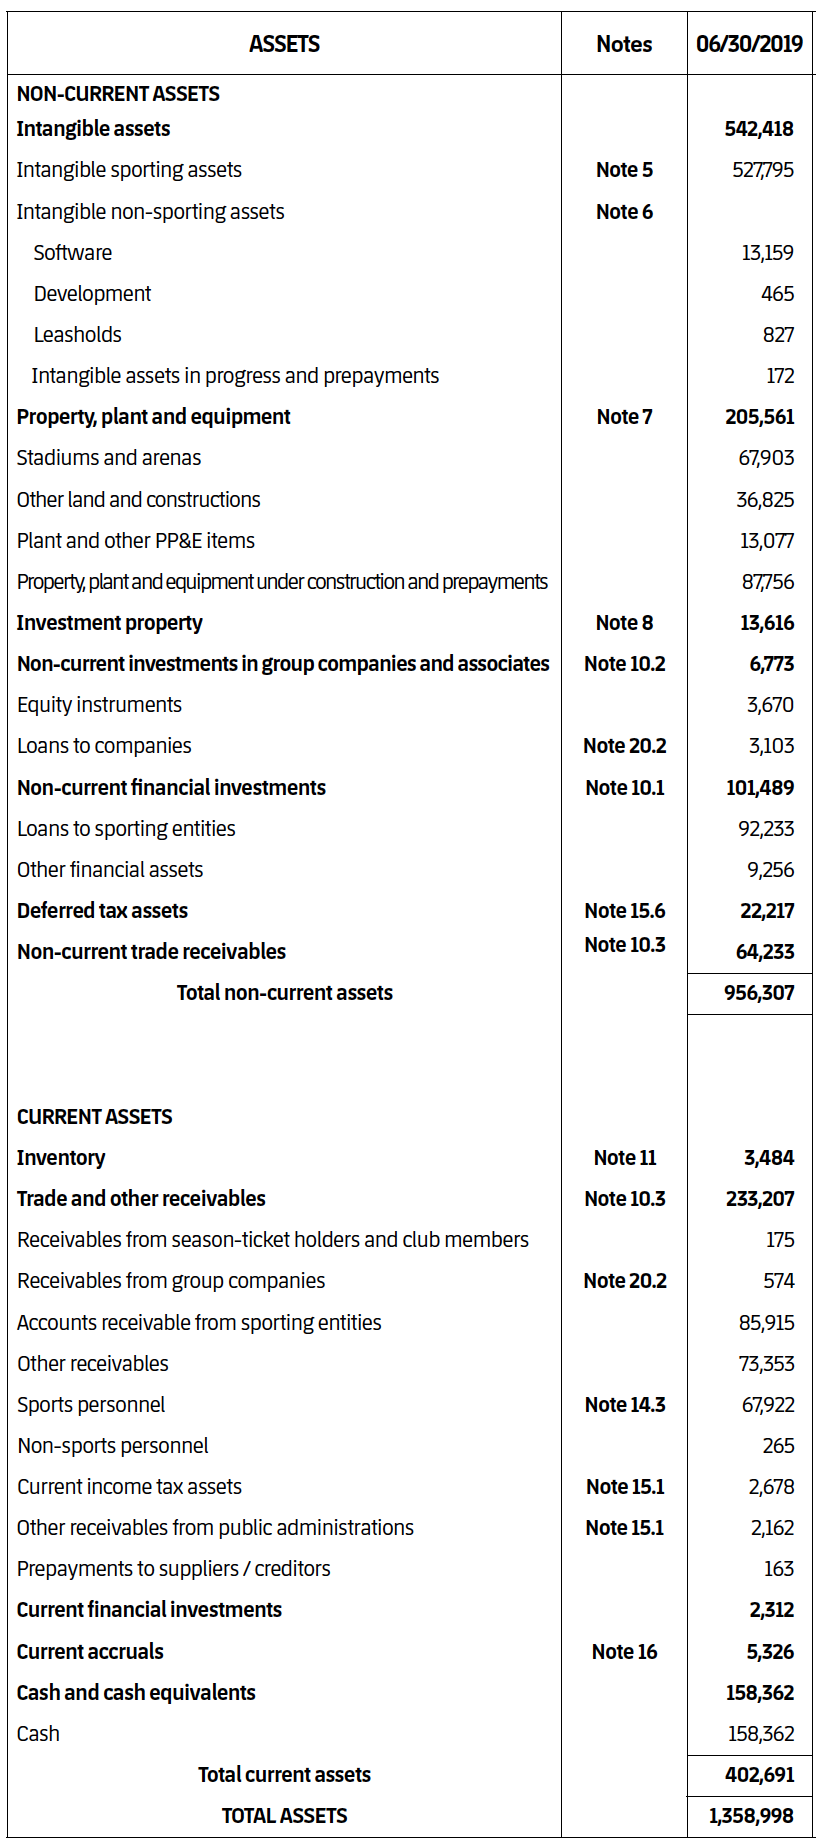
\includegraphics[width=.45\textwidth]{img/SP_attivo_barca.png} \label{sp_attivo_barca}} \quad
            \subfloat[][Stato Patrimoniale passivo al 30 Giugno 2019]
            {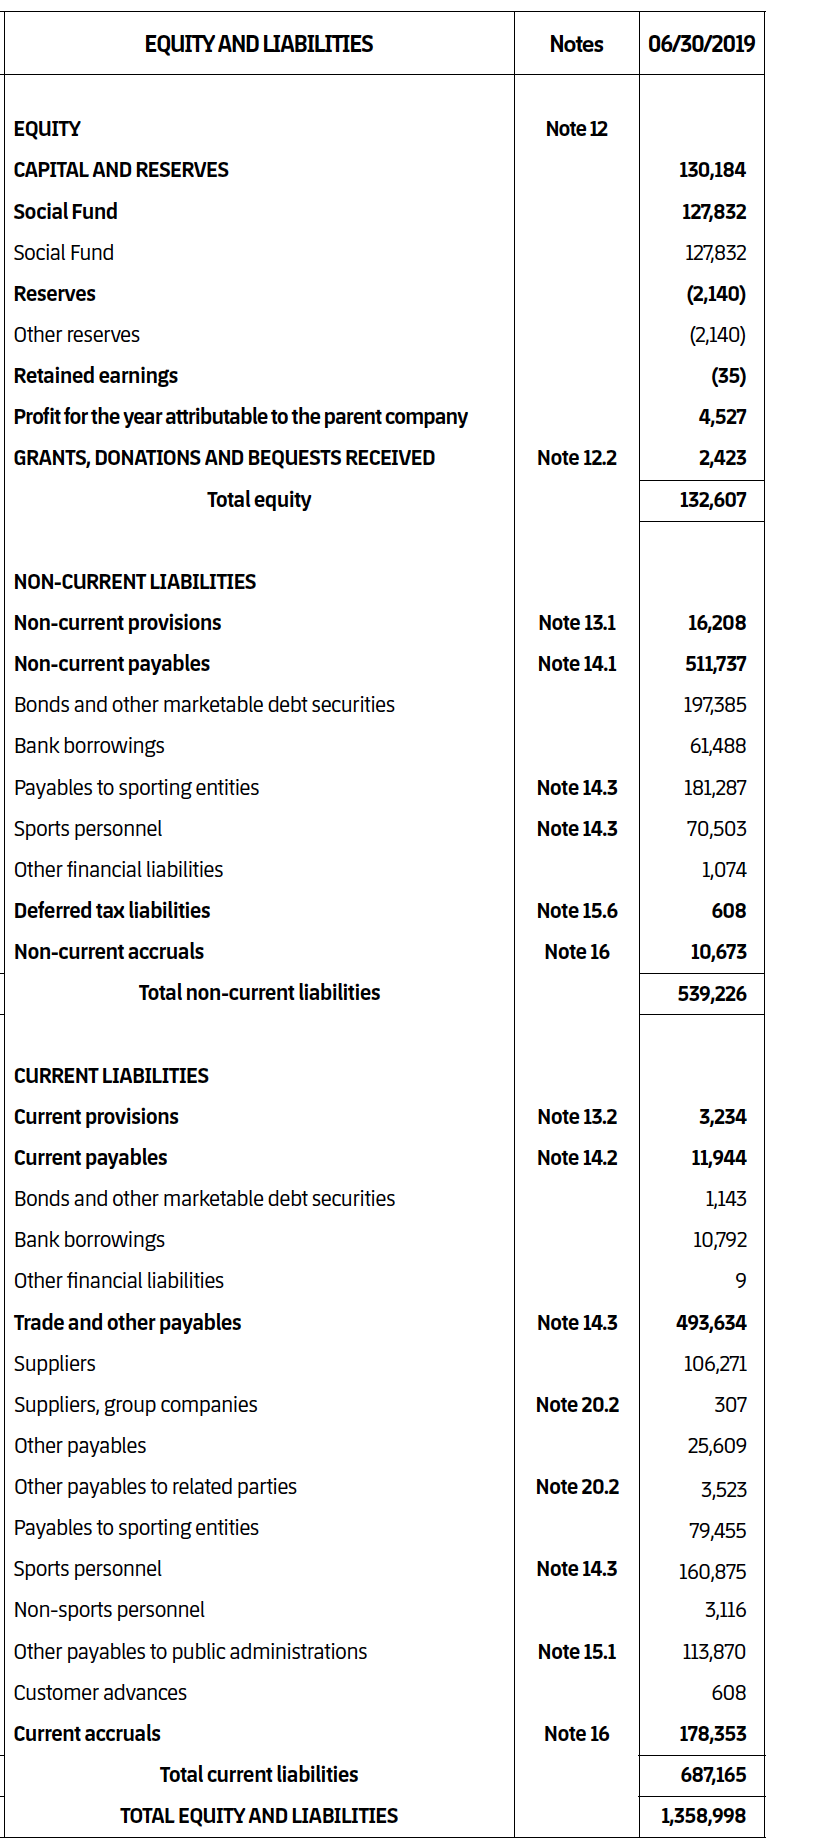
\includegraphics[width=.45\textwidth]{img/SP_passivo_barca.png} \label{sp_passivo_barca}}
            \caption{Stato Patrimoniale Barcellona al 30 Giungno 2019}
            \label{sp_barca}  
        \end{figure}
        \begin{equation}
                \text{Margine di Tesoreria} = 399.207.000-687.165.000 = \mathbf{-287.958.000\mbox{\euro}}
            \label{eqn: marg_teso_barca}
        \end{equation}
        \begin{equation}
                \text{Indice di liquidit\'a primaria} = \frac{399.207.000}{687.165.000} = \mathbf{58,09\%}
            \label{eqn: ind_liq_barca}
        \end{equation}
       Dopo una prima analisi positiva torniamo ora ad affrontare una sezione pi\'u complessa: l'indice di liquidit\'a primario
       che esprime in percentuale il margine di tesoreria mostra come circa la met\'a delle passivit\'a a breve termine sia scoperta dalle
       liquidit\'a disponbili, andando a creare un problema nel caso serva ripagare le passivit\'a a breve termine.
    \item Analisi della solidit\'a:\newline
        \begin{equation}
            \text{Grado di Indipendenza Finanziaria} = \frac{132.607.000}{1.358.998.000} = \mathbf{9,7\%}
        \label{eqn: indeb_barca}
        \end{equation}
        \begin{equation}
            \text{Margine di Struttura} = 132.607.000-747.979.000 = \mathbf{-615.372.000\mbox{\euro}}
        \label{eqn: marg_strutt_barca}
        \end{equation}
        Anche la solidit\'a della societ\'a non produce risultati molto soddisfacenti: il patrimonio netto non finanzia neanche il 10\% 
        delle passivit\'a totali, mentre le immobilizzazioni risultano "scoperte" per pi\'u di 600mln€. Questi risultati evidenziano come
        la societ\'a faccia uso quasi nella totalit\'a al capitale di debito.\newpage
    \item Analisi della Redditivit\'a:\newline
        \begin{equation}
            \text{ROI} = \frac{17.542.000}{1.358.988.000} = \mathbf{1,29\%}
        \label{eqn: roi_barca}
        \end{equation}
        \begin{equation}
            \text{ROE} = \frac{23.501.000}{354.919.000} = \mathbf{6,62\%}
        \label{eqn: roe_barca}
        \end{equation}
        Confrontando invece voci economiche e patrimoniali i risultati cambiano: il risultato operativo rimane positivo grazie ai risultati sportivi
        raggiunti e ad alcune operazioni di mercato che hanno alleggerito in modo minimo le casse del club, rendendo quindi il ROI positivo 
        ma molto vicino allo 0; il ROE invece ha un valore positivo e maggiore di 0 andando quindi a mostrare come, seppur pochi, investimenti 
        fatti con i mezzi propri siano buoni.
\end{enumerate}
\subsection{Manchester City}
Come ultimo club di questa prima parte della trattazione andremo a vedere il Manchester City, squadra di grande peso in Inghilterra anche se,
come \'e accaduto con il Paris Saint Germain, solo grazie all'acquisto del club da parte di sceicchi in grado di effettuare grandi investimenti 
senza troppe preoccupazioni sul ritorno. Dalla sua fondazione, nel 1894, fino al 2008 (anno dell'approdo degli sceicchi in Premier League) i \emph{Citizens} "ventavano"
un bacheca contenente: 2 campionati inglesi, 4 coppe d'inghilterra, 2 coppe di lega inglesi, 3 Community Shield e 1 Coppa delle Coppe. 
In soli 10 anni invece \'e riuscita a conquistare: 4 campionati inglesi, 2 coppe d'inghilterra, 4 coppe di lega e 3 Community Shield\footnote{https://it.wikipedia.org/wiki/Manchester\_City\_Football\_Club\#Palmar\%C3\%A8s}.\newpage
\begin{enumerate}
    \item Analisi dei Ricavi:\newline
        \begin{figure}
            \centering
            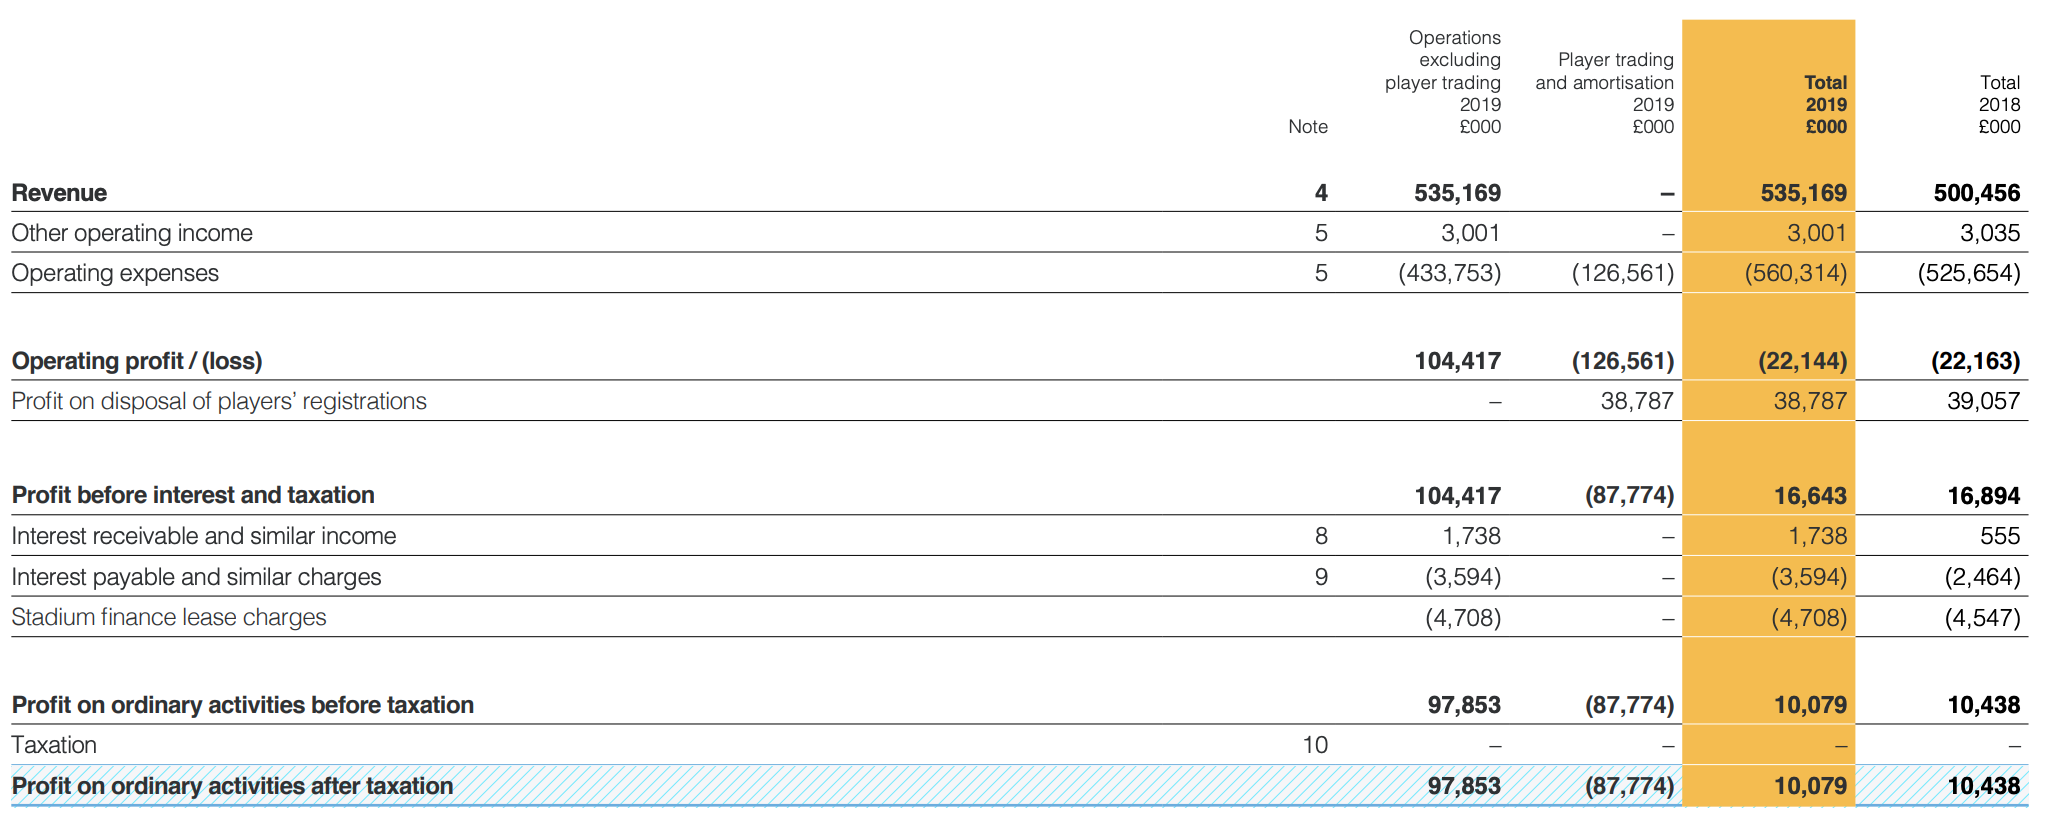
\includegraphics[scale=.4]{img/CE_city.png}
            \caption{Conto Economico Manchester City al 30 Giugno 2019}
            \label{ce_city}
        \end{figure}\newline
        \begin{equation}
            \frac{\text{Ricavi da gare}}{\text{Totale Ricavi}} = \frac{55.007.000}{535.169.000} = \mathbf{10,27\%}
            \label{eqn: gare_city}
        \end{equation}
        \begin{equation}
            \frac{\text{Diritti TV}}{\text{Totale Ricavi}} = \frac{253.176.000}{535.169.000} = \mathbf{47,30\%}
            \label{eqn: tv_city}
        \end{equation}
        \begin{equation}
            \frac{\text{Ricavi commerciali}}{\text{Totale Ricavi}} = \frac{228.833.000}{535.169.000} = \mathbf{42,75\%}
            \label{eqn: commerc_city}
        \end{equation}
        Dal punto di vista dei ricavi, la societ\'a pu\'o giovare di due grandi propriet\'a del calcio inglese: essere uno dei campionati
        pi\'u seguiti al mondo e di conseguenza avere fan in giro per il mondo che contribuiscono all'acquisto dei prodotti de club. Per questo 
        motivo i ricavi commerciali e quelli da diritti tv sono molto elevati e compongono la quota maggiore sul totale. I ricavi da gare
        rimangono in percentuale stabili.\newpage
    \item Analisi della liquidit\'a:\newline
        \begin{figure}
            \centering
            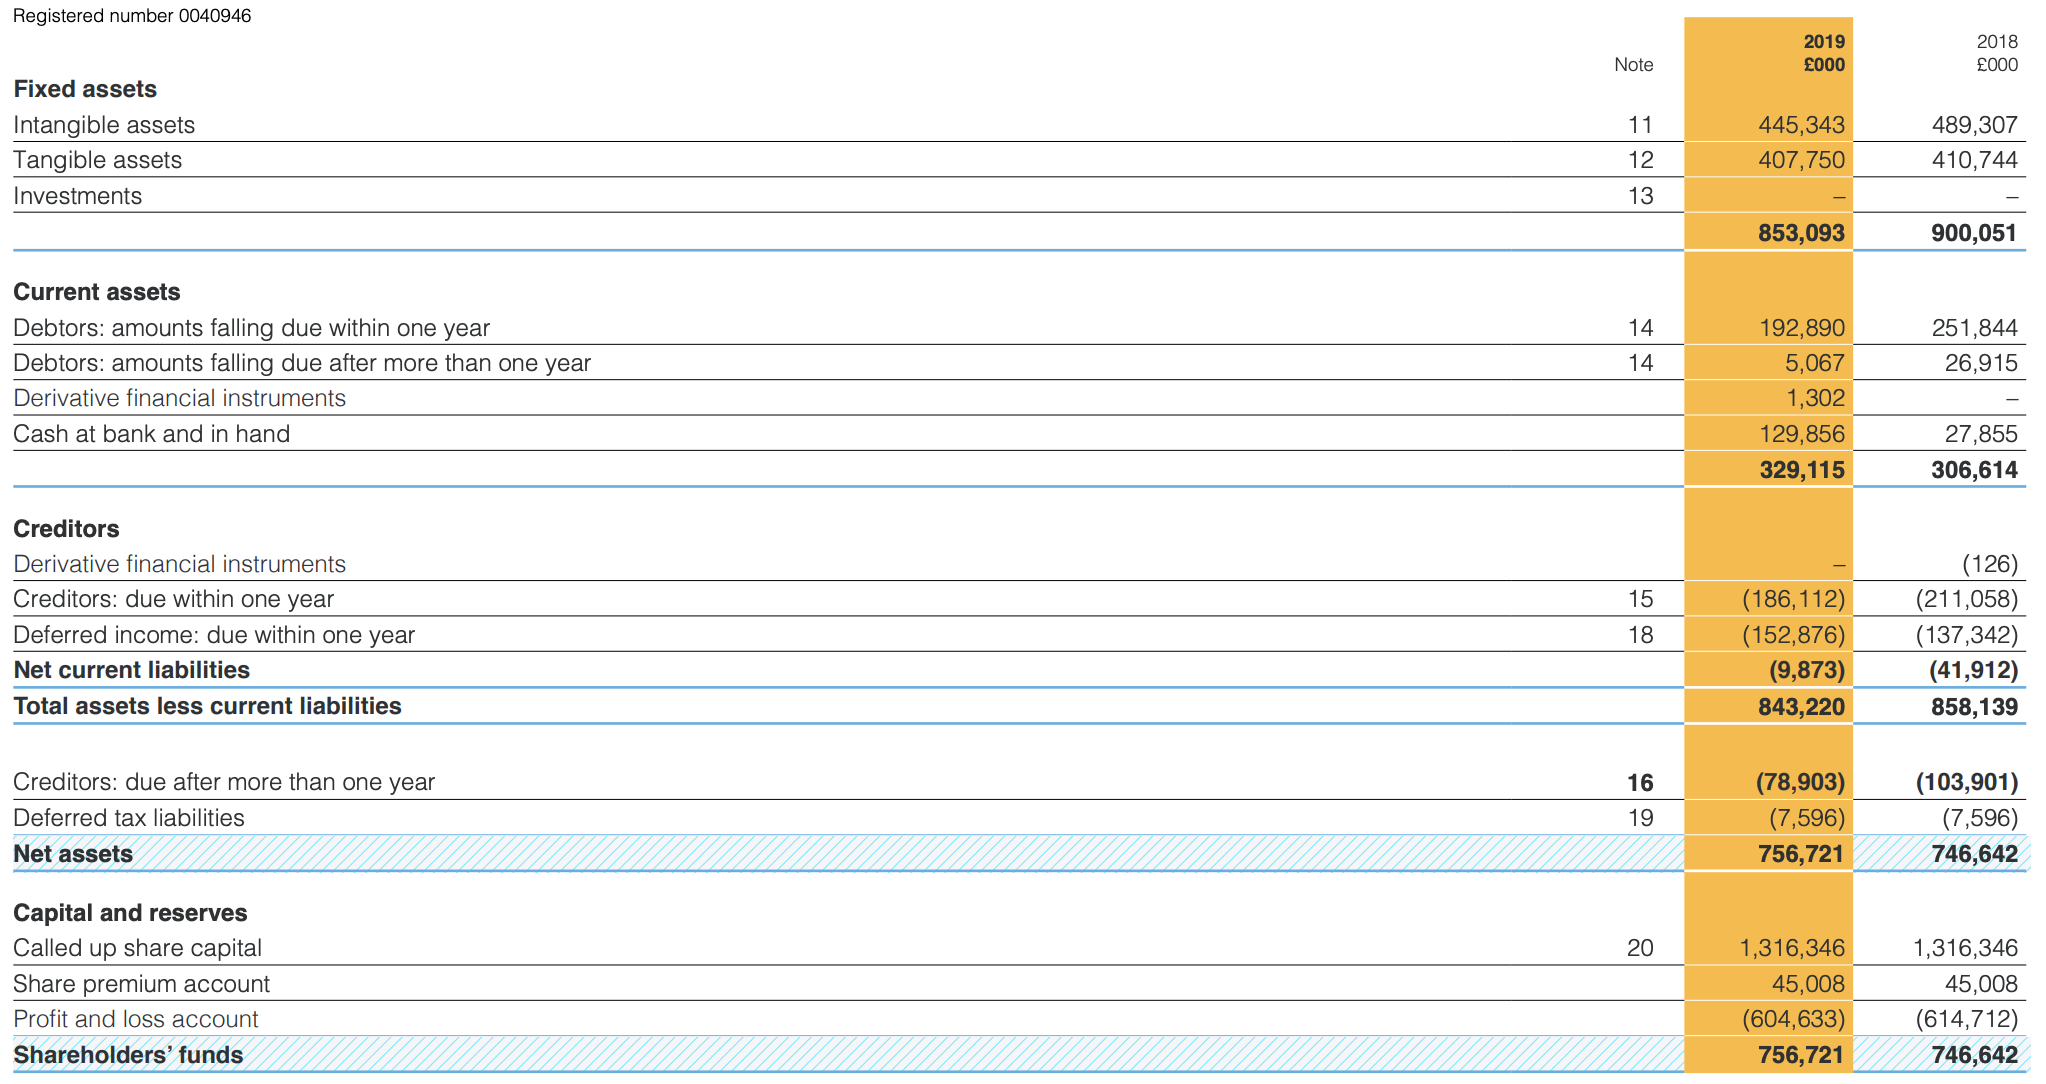
\includegraphics[scale=.4]{img/SP_city.png}
            \caption{Stato Patrimoniale Manchester City al 30 Giugno 2019}
            \label{sp_city}
        \end{figure}\newline
        \begin{equation}
                \text{Margine di Tesoreria} = 129.856.999 - 843.220.000 = \mathbf{-713.364.000\pounds}
            \label{eqn: marg_teso_city}
        \end{equation}
        \begin{equation}
                \text{Indice di liquidit\'a primaria} = \frac{129.856.999}{843.220.000} = \mathbf{15,40\%}
            \label{eqn: ind_liq_city}
        \end{equation}
        Anche in questo caso troviamo uno scenario simile a quello del Barcellona. Se da un lato i ricavi possono avere il loro significato 
        mostrando come una societ\'a produca effettivamente risultati nel breve periodo, dal punto di vista patrimoniale non si pu\'o dire 
        lo stesso: le passivit\'a a breve termine sono scoperte per quasi la totalit\'a del loro valore, solo il 15\% potr\'a essere 
        coperto con denaro liquido e disponibile sin da subito.
    \item Analisi della solidit\'a:\newline
        \begin{equation}
            \text{Grado di Indipendenza Finanziaria} = \frac{756.721.000}{1.182.208.000} = \mathbf{64,00\%}
        \label{eqn: indeb_city}
        \end{equation}
        \begin{equation}
            \text{Margine di Struttura} = 756.721.000 - 853.093.000 = \mathbf{-96.372.000\pounds}
            \label{eqn: marg_strutt_city}
        \end{equation}
        Per quanto riguarda la solidit\'a troviamo un grado di indipendenza finanziaria positivo, stando a significare un buon grado di autonomia
        rispetto ai finanziatori esterni. Il margine di struttura evidenzia come le immobilizzazioni (materiali, immateriali e finanziarie) non 
        siano per\'o completamente coperte dal Patrimonio Netto, con uno scoperto comunque accettabile pari a meno di 100mln£.
    \item Analisi della Redditivit\'a:\newline
        \begin{equation}
            \text{ROI} = \frac{-22.154.000}{1.182.208.000} = \mathbf{-1,81\%}
        \label{eqn: roi_city}
        \end{equation}
        \begin{equation}
            \text{ROE} = \frac{10.079.000}{756.721.000} = \mathbf{1,33\%}
        \label{eqn: roe_city}
        \end{equation}
        Anche nell'ultima parte di analisi i risultati non sono molto consistenti. Se si considera il risultato operativo esclusi 
        i ricavi dallo scambio dei giocatori, da un profitto si arriva ad una perdita, a dimostrazione di come sia importante e pesante
        il business dei calciatori e dei loro cartellini. Il ROE, invece, che considera il risultato netto, si "salva" grazie ai profitti
        sulla cessione di registrazione dei calciatori che elimina la perdita generata con la sola sottrazioen di ricavi e costi.
\end{enumerate}
\chapter{Fair Play Finanziario}
\section{Dalla nascita alle ultime riforme}
Il \textbf{Fair Play Finanziario} \'e un insieme di norme emanate dalla UEFA che cercano di porre rimedio alla molto negativa situazione economico-
finanziaria del sistema calcio, generatasi a partire dall'inizio degli anni 90 e che ancora oggi, come abbiamo avuto modo di analizzare, non 
\'e stata del tutto risolta.
Questa idea \'e nata in seguito ad una indagine condotta dalla UEFA nel 2010 su pi\'u di 600 Club in Europa. 
L'analisi mostrava come pi\'u della met\'a dei Club coinvolti, e di questa fetta la maggior parte erano di grandi dimensioni, 
presentava ingenti perdite d'esercizio. Da quel momento la Federazione decise che si dovesse intevenire in qualche modo e inizialmente
concentrarono il loro studio su 3 macro-aree:
\begin{enumerate}
    \item \textbf{Debiti scaduti non pagati};
    \item \textbf{Incidenza del costo del lavoro sul totale dei ricavi};
    \item \textbf{Rapporto squilibrato tra ricavi e costi}.
\end{enumerate}
In seguito ad aver riconosciuto le aree in cui fosse necessario migliorare \'e stata presa la decisione di redigere, il 27 Maggio 2010, la 
\textbf{\emph{Uefa Club Licensing and Financial Fair Play Regulation}} in accordo con tutte le societ\'a europee.
Il documento prevede degli obiettivi di carattere sociale e di crescita collettiva ma anche, ovviamente, economico\footnote{UEFA: https://documents.uefa.com/v/u/MFxeqLNKelkYyh5JSafuhg}:
\begin{enumerate}[(a)]
    \item Promuovere ulteriormente e migliorare continuamente il livello di tutti gli aspetti del
    del calcio in Europa e a dare costante priorità alla formazione e alla cura dei
    giovani giocatori in ogni club; 
    \item Assicurare che i club abbiano un livello adeguato di gestione e organizzazione;
    \item Adattare le infrastrutture sportive dei club per fornire a giocatori, spettatori e rappresentanti dei media
    strutture adeguate, ben attrezzate e sicure;
    \item Proteggere l'integrità e il regolare svolgimento delle competizioni UEFA per club;
    \item Permettere lo sviluppo del benchmarking per i club in termini di criteri finanziari, sportivi, legali,
    legali, personali, amministrativi e infrastrutturali in tutta Europa.
    \item Migliorare la capacità economica e finanziaria dei club, aumentando la loro
    trasparenza e credibilità;
    \item Dare l'importanza necessaria alla protezione dei creditori e garantire
    che i club saldino puntualmente i loro debiti con i dipendenti, le autorità sociali/fiscali e gli altri
    club in modo puntuale;
    \item Introdurre più disciplina e razionalità nelle finanze del calcio dei club;
    \item Incoraggiare i club ad operare sulla base delle proprie entrate;
    \item incoraggiare la spesa responsabile per il beneficio a lungo termine del calcio;
    \item Proteggere la redditività e la sostenibilità a lungo termine del calcio europeo per club.
\end{enumerate}
Entrando più nello specifico, la UEFA ha dovuto introdurre alcune misure specifiche per fare in modo che i club entrassero in questa nuova 
mentalit\'a di \textbf{spendere solo i soldi che si hanno}, puntando quindi ad un obiettivo di \textbf{pareggio di bilancio} e \textbf{
controllo dei costi}. Il primo punto che le societ\'a hanno dovuto tenere sotto controllo dal momento in cui il Fair Play Finanziario \'e entrato in vigore, 
sono le entrate: essendo uno dei due fattori (Costi-Ricavi) che permettono di arrivare ad un punto di equilibrio hanno dovuto porre maggior impegno su di esse. 
Se si osserva infatti il totale dei ricavi generati dalle principali squadre europee dal 2010 ad oggi (2019) si pu\'o notare quanto segue:
\begin{figure}
    \centering
    \subfloat[][Ricavi all'anno 2010]
    {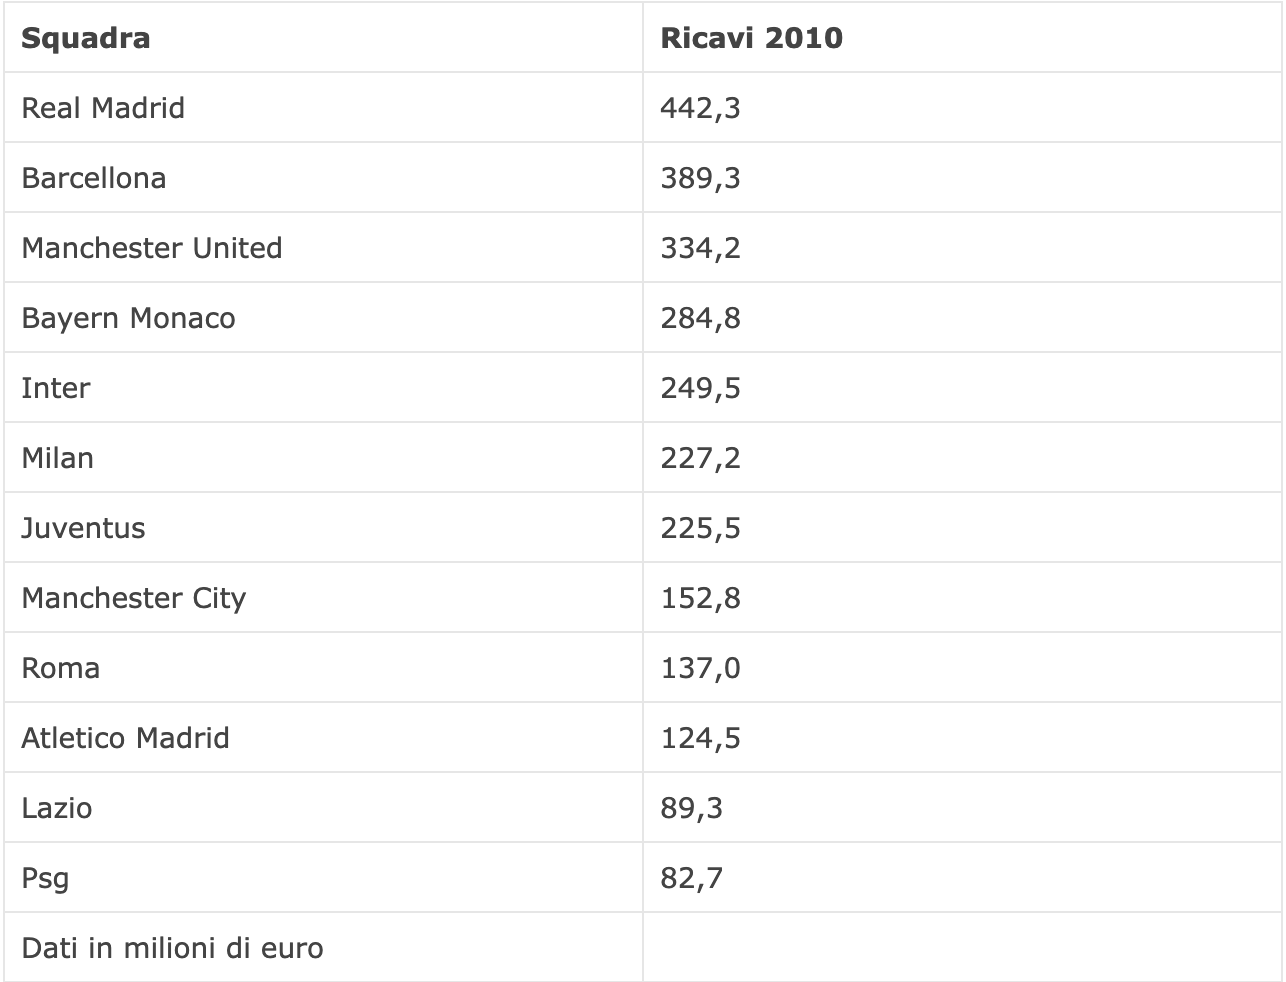
\includegraphics[width=.35\textwidth]{img/ricavi_2010.png} \label{ricavi_2010}} \quad
    \subfloat[][Ricavi all'anno 2019]
    {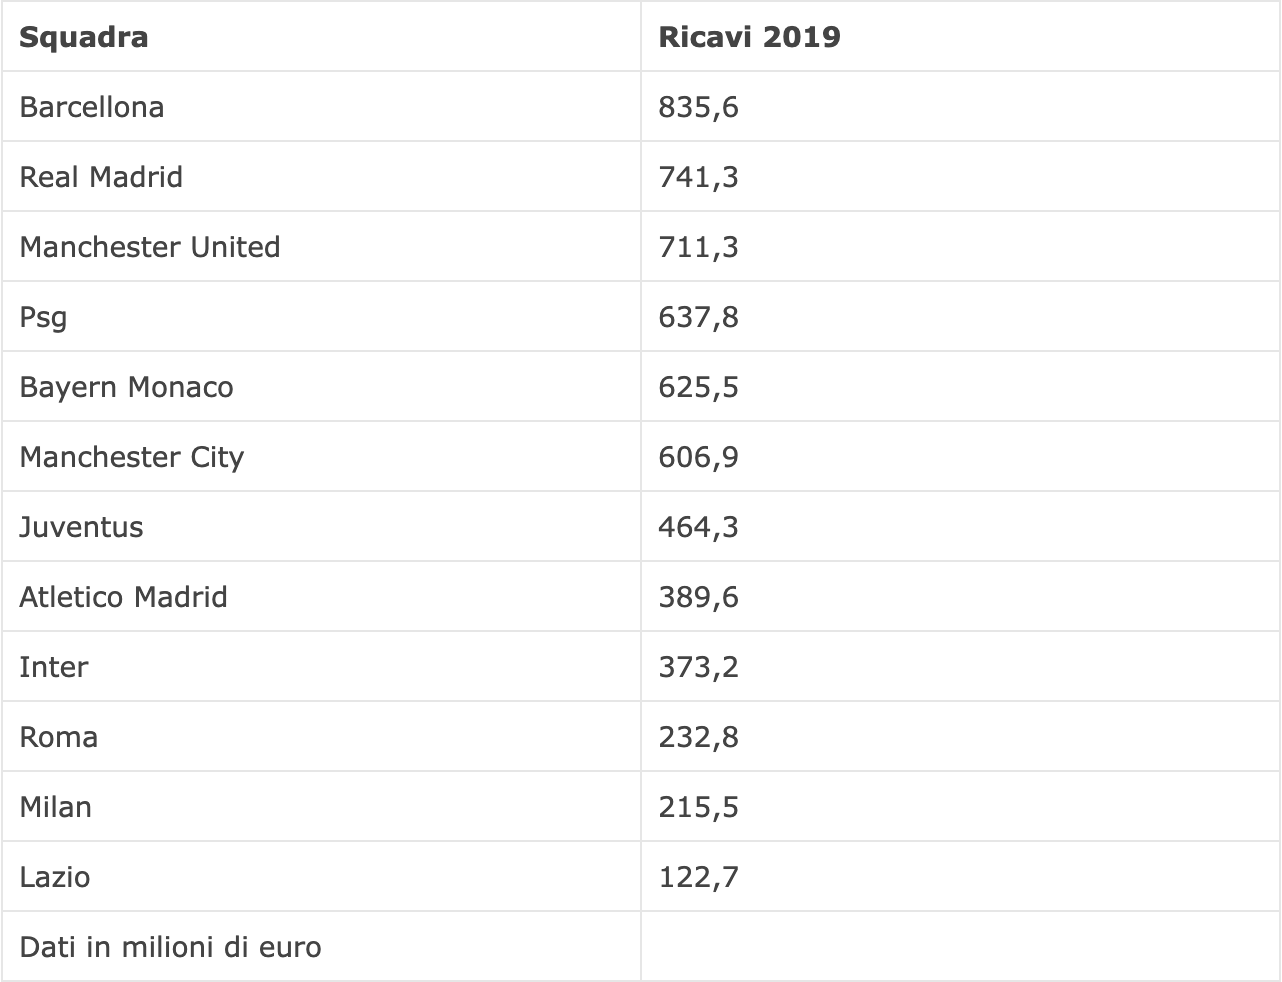
\includegraphics[width=.35\textwidth]{img/ricavi_2019.png} \label{ricavi_2019}}
    \caption{Comparazione ricavi 2010-2019}
    \label{comp_ricavi_10_19}  
\end{figure}
La figura \ref{comp_ricavi_10_19}\footnote{https://www.calcioefinanza.it/2019/12/30/classifica-ricavi-squadre-decennio-juve-inter-milan/}
spiega come in seguito all'approvazione del \emph{FFP} i principali club europei hanno captato la necessit\'a di modificare qualcosa nel loro core business,
sopratutto per quanto riguarda la voce dei ricavi da gare, ricavi da diritti televisivi e ricavi commerciali\footnote{Analisi presente nel Capitolo Uno}.
L'incremento maggiore \'e stato quello del Paris Saint Germain che ha registrato un +671.2\%, certamente
grazie all'approdo degli sceicchi alla dirigenza; nelle posizione successive troviamo i principali Club di Germania, Inghilterra e Spagna
con incrementi superiori al 100\%; solo nelle ultime posizioni troviamo nomi italiani, con al primo posto la Juventus che ha vissuto un aumento 
poco superiore al 100\%. Per ultima, la societ\'a AC Milan che ha subito addirittura un decremento rispetto al 2010,
a causa di un periodo buio in quanto a risultati sportivi a partire proprio da quell'anno, che hanno portato meno tifosi allo stadio ma sopratutto meno incassi 
da diritti televisivi.\newline
Questo rinnovato interesse delle societ\'a rispetto a questi aspetti che coinvolgono in misura considerevole il consumatore finale, ha fatto
si che fosse proprio quest'ultimo ad approfittarne, andando per esempio a rendere la partita allo stadio come
un momento da vivere a 360 gradi che ti deve coinvolgere dal momento in cui entri al momento in cui esci.\newline
Uno dei pilastri principali economici su cui i basa il \emph{Fair Play Finanziario} \'e la \emph{\textbf{Break-Even Rule}}.
Essa viene articolata a partire dall'articolo 57 del documento e specifica come le squadre che vogliano partecipare a competizioni UEFA debbano
rispettare il pareggio di bilancio e altre regolamentazioni di tipo economico-finanziarie. Il rispetto di queste regole per\'o si basa su 
un \emph{monitoring period}, cio\'e un periodo di monitoraggio durante il quale la Federazione effettua dei controlli per poter arrivare in seguito 
ad un giudizio ponderato e corretto. Il periodo di monitoraggio si basa sui 2 esercizi precedenti a quello preso in considerazione pi\'u quello attuale.
Al termine dell'analisi non si deve aver infranto nessuno dei punti presenti poi all'Articolo 62 parte 3, al cui interno 
\'e compresa anche la \emph{Break-Even Rule}. Vi sono per\'o delle condizioni in cui \'e possibile infrangere uno dei punti della parte 3 
ed essere ugualmente in grado di soddisfare i requisiti per ottenere la licenza UEFA:
\begin{enumerate}
    \item Il club che presenta la richiesta per la licenza deve aver conseguito un utile nei tre periodi precedenti all'analisi;
    \item Il club che richiede la licenza presenta una perdita ma all'interno del margine delineato all'interno dell'art. 61 parte 2\footnote{Massimo 5 milioni di euro oppure 30 milioni in caso la perdita sia contenuta con contributi delle partecipate e/o parti correlate}
\end{enumerate}
Per poter spiegare in modo pi\'u concreto il significato della \emph{Break-Even Rule} \'e necessario capire come arrivare al punto di pareggio.
In Economia, il punto di pareggio (\emph{Break-Even Point}) viene identificato tramite la quantit\'a da vendere necessaria a coprire i costi 
sostenuti per la produzione, per poter terminare il periodo senza perdite o profitti. Anche in questo caso la regola applicata \'e la stessa,
ma per la UEFA \'e necessario considerare solo i \textbf{Ricavi Rilevanti} e i \textbf{Costi Rilevanti}.
\newpage
\begin{table}
    \begin{tabularx}{\textwidth}{XX}
        \toprule
        \textbf{Ricavi Rilevanti} & \textbf{Costi Rilevanti} \\
        \midrule
        Ricavi da gare & Costi dei materiali (voce che comprende tutti gli aspetti dell'attivit\'a sportiva) \\
        \midrule
        Ricavi da diritti TV & Costo del personale \\
        \midrule
        Sponsor e pubblicit\'a & Costi per organizzazione gare e affitto impianti sportivi \\
        \midrule
        Ricavi commerciali & Ammortamenti e svalutazioni relative ai calciatori \\
        \midrule
        Ricavi da cessione calciatori & Gli oneri finanziari e dividendi \\
        \midrule
        Ricavi da cessione di immobilizzazioni & \\
        \bottomrule
    \end{tabularx}
    \caption{Tabella Costi e Ricavi Rilevanti}
    \label{tabella_ric_costi_ril}
\end{table} 
Tramite la tabella \ref{tabella_ric_costi_ril} \'e possibile capire in modo pi\'u immediato cosa racchiudono queste due voci. La voce principale 
che non viene considerata per il calcolo del \emph{Break-Even} \'e quella realtiva al settore giovanile, che essendo eslusa da queste regole
permette ai club di investire senza dover pensare ad alcun tipo di regola, permettendogli cos\'i di generare un potenziale ritorno
elevatissimo. L'esempio pi\'u lampante di societ\'a che ha accolto in modo positivo questa norma \'e l'Ajax, squadra olandese famosa in 
tutto il mondo perch\'e capace ogni anno di produrre talenti dal settore giovanile per poi venderli successivamente
producendo plusvalenze notevolissime.\newline
In conclusione, quindi, i criteri di base per il rispetto del \emph{Fair Play Finanziario} non sono fondamentalmente complicati, ma, come 
si potr\'a vedere successivamente non tutte le societ\'a sono state in grado di rispettarlo.
\subsection{Le riforme del 2014, del 2015 e del 2018}
Cos\'i come inizialmente impostato, il documento prevedeva sostanzialmente una limitazione alla libert\'a di spesa da parte dei club. 
I pi\'u facoltosi tra di essi accusavano la Federazione di, tramite l'introduzione della \emph{Break-Even Rule}, non permettergli di 
esercitare la loro attivit\'a in maniera completamente libera. Sempre pi\'u societ\'a si sono unite a questa corrente di pensiero,
fino ad arrivare nel 2014 ad una vera e propria citazione in giudizio: a seguito di una multa ai danni del Manchester City di 49 milioni di sterline per aver infranto 
le regole del FFP, l'avvocato Jean–Louis Dupont port\'o il fatto davanti al \emph{Tribunal de Première Istance de Bruxelles} dove quest'ultimo pass\'o la disputa alla 
Corte di Giustizia che a sua volta port\'o la UEFA ad dover deferire alcuni punti del documento\footnote{Calcio e Finanza: https://www.calcioefinanza.it/2015/06/23/fair-play-finanziario-dupont-sospensione/}.\newline
La prima grande modifica \'e avvenuta sempre nel 2014, tramite l'introduzione del \textbf{Settlement Agreement}, inserito all'interno dell'articolo 68 e il quale permette
ai club di avanzare una richiesta di "abbuono" delle sanzioni nel caso in cui questi ultimi si rendano conto di non riuscire a rispettare le regole del 
\emph{Break-Even}. Questo accordo si basa su alcuni punti che possono influenzare il rispetto o meno di questo "paletto" e quindi considerabili
come una sorta di giustificazione\footnote{Allegato XI del documento sul \emph{Financial Fair play}}:
\begin{enumerate}
    \item Il quantum e l’andamento del Break-even Result;
    \item La proiezione aggregata del Break-even Result;
    \item L’incidenza del cambio della valuta locale in euro;
    \item La posizione debitoria;
    \item Cause di forza maggiore, per esempio circostanze oltre il controllo del club;
    \item Grossi ed imprevedibili cambiamenti nel mondo economico;
    \item Il fatto di operare in un mercato inefficiente;
    \item Il limite di giocatori imposto dalle licenze
\end{enumerate}
Nel caso quindi si verifichi uno di questi scenari oppure venga provato come uno di questi punti abbia impedito al club di rispettare le 
regole del FFP, \'e possbile richidere una estensione del \emph{monitoring period} per rientrare nei termini ed evitare 
sanzioni pi\'u pesanti.\newline
L'anno succesivo, nel 2015, \'e stata introdotta una ulteriore modifica al documento. Insieme al \emph{Settlement Agreement} la nuova riforma
prevedeva la possibilit\'a di stipulare un \emph{\textbf{Voluntary Agreement}}. Sostanzialmente l'accordo prevede che un club possa usufruire di una
deroga ai limiti di spesa imposti dal \emph{FFP} per una stagione sportiva. Se il punto di partenza del \emph{Settlement Agreement} era il
club stesso che poteva chidere pene meno severe in caso di non rispetto degli obblighi di pareggio, in questo caso \'e la federazione che
propone una soluzione alle societ\'a per rientrare nei limiti. L'accordo \'e contenuto all'interno dell'articolo 57 del documento e prevede 
che il club a cui viene proposto questo patto debba presentare una sorta di \emph{Business Plan} in cui eventuali flussi di cassa futuri 
giustifichino la spesa superiore e quindi la violazione del \emph{Break-Even}. Inoltre la stipulazione del \emph{Voluntary Agreement} \'e
subordinata al rispetto di alcuni punti:
\begin{itemize}
    \item Nella stagione precedente il club che ha richiesto l'accordo non deve aver conquistato una posizione valevole per le coppe
    europee ma \'e riuscito ad ottenere la licenza UEFA dalla Federazione nazionale;
    \item Nell’anno in cui viene fatta richiesta per il Voluntary agreement il club gioca una competizione europea ed è in regola con
    le regole del FFP;
    \item Il club che richiede l'accorod deve aver subito un cambio sostanziale nella propriet\'a o negli organi di controllo, nei 12 mesi 
    precedenti alla richiesta;
    \item Il club che richiede l'accordo non deve aver richiesto negli ultimi tre esercizi un altro tipo di accordo con la Federazione;
    \item Il club non deve aver subito una sanzione da parte dell'Organo di Controllo FInanziario della UEFA.
\end{itemize}
Nel caso in cui la Federazione accetti questo \emph{Business Plan} di medio-lungo periodo, la societ\'a sar\'a giustificata per il non 
rispetto delle regole del \emph{FFP}.\newline
L'ultima riforma pi\'u significativa attuata dalla UEFA nella regolamentazione del \emph{Fair Play Finanziario} \'e avvenuta nel 2018.
Quest'ultima modifica, che ha dato vita a quello che verr\'a poi chiamato \emph{\textbf{Fair Play Finanziario 2.0}}, si basa sulla volont\'a della
UEFA di voler porre fine ad alcune strategie effettuate dai club per eludere le regole. In particolare i punti 
salienti di questa modifica sono\footnote{Gazzetta dello Sport: https://www.gazzetta.it/Calcio/24-05-2018/fair-play-altro-giro-vite-uefa-vara-nuove-regole-270362431241.shtml}:
\begin{itemize}
    \item I club saranno obbligati rendere note tutte le informazioni econico finanziarie (pubblicazione online dei bilanci) e 
    sopratutto sar\'a obbligatorio esprimere le spese per gli agenti sportivi;
    \item Possibilit\'a di controllo e di applicazione delle sanzioni in modo immediato in caso di sospette violazioni del \emph{FFP};
    \item Non sarà più possibile comprare un giocatore «fingendo» un prestito, per posticipare il deficit. L’operazione andrà iscritta 
    a bilancio come acquisto in modo immediato;
    \item Non sar\'a pi\'u possibile vendere giocatori ad un club con lo stesso proprietario per ridurre il debito;
    \item Gli incassi potranno essere contabilizzati quando effettivamente realizzati (principio di competenza economica);
    \item Controlli pi\'u serrati su: posizione debitoria e gestione del deficit.
\end{itemize}
Anche se pochi, questi punti hanno dato un'ulteriore stretta alle possibilit\'a delle societ\'a di evitare le punizioni imposte dalla federazione,
cercando quindi di creare un nuovo "inizio" del calcio europeo.\newline
Le modifiche, quindi, non sono state poche durante questi ultimi anni. Le societ\'a, per\'o, anche se tenute sempre pi\'u attentamente
sotto sorveglianza sono riuscite in molti casi ad eludere le sanzioni, e come avremo modo di capire anche grazie alla Federazione stessa.
\section{Favoritismi verso alcuni club}
Se da un lato l'introduzione del \emph{Fair Play Finanziario} ha generato una diminuzione del debito globale del sistema calcio,
passando da -1.163 milioni di euro nel 2009 ad addirittura un risultato positivo aggregato di 140 milioni di euro nel 2018\footnote{Calcio e Finanza: https://www.calcioefinanza.it/2020/03/02/fair-play-finanziario-e-plusvalenze-fittizie-alcune-possibili-soluzioni/};
dall'altro lato ha generato molti dubbi da parte degli appassionati ma anche di alcune societ\'a. Durante questi 12 anni passati dall'
introduzione di queste regole, le squadre sanzionate non sono state poche: sono 43 le squadre che in totale hanno ricevuto delle penalit\'a
da parte della UEFA, di queste, 16 sono state estromesse dalle competizioni europee per uno o pi\'u anni, mentre 27 hanno sottoscritto il 
\emph{Settlement Agreement}\footnote{Sport Mediaset: https://www.sportmediaset.mediaset.it/calcio/calcio/uefa-e-fair-play-finanziario-ecco-i-club-sanzionati-in-passato\_1215471-201802a.shtml}. 
Nonostante il numero non sia tutt'altro che basso, non sono mancati alcuni casi in cui le sanzioni sarebbero state da
applicare ma per alcuni motivi non troppo chiari non \'e state avviata alcun tipo di procedura oppure sono state applicati criteri diversi per
scenari simili.\newline
Il primo esempio pratico \'e riconducibile al \textbf{Manchester City}, squadra che come analizzato in precedenza ha vissuto una crescita esponenziale
sia in termini economici che in termini di risultati sportivi, dal momento dell'acquisto del club da parte dei magnati arabi. I primi problemi
iniziano nel 2014 quando, a seguito dei controlli della UEFA in merito al rispetto della \emph{Break-Even Rule} sono state contestate alcune irregolarit\'a.
Il risultato delle indagini \'e stato che i bilanci del 2011/2012 e 2012/2013 non rispettavano la suddetta regola. Il 16 maggio del 2014 il club sigl\'o con la Federazione
un \emph{Settlement Agreement}, il cui contenuto prevedeva:
\begin{itemize}
    \item Una multa di 60 milioni di euro;
    \item La limitazione della rosa a 21 giocatori nelle competizioni europee, di cui 8 cresciuti nel vivaio del club;
    \item L’impegno al raggiungimento del pareggio di bilancio in un orizzonte temporale prestabilito;
    \item Chiudere l’esercizio 2013/14 con una perdita di bilancio di massimi di 20 milioni di euro;
    \item Chiudere l’esercizio 2014/15 con una perdita di bilancio di massimi 10 milioni di euro nell’esercizio 2014/15;
    \item Il Manchester City si impegna inoltre con Nyon a non incrementare il costo della rosa nelle stagioni 2014/15 e 2015/16.
\end{itemize}
Quest'ultimo punto non sarebbe stato considerato nel caso di rispetto dell'accordo nei termini di risultato netto. \newline
La voce che impattava in modo maggiore sul non pareggio di bilancio sono stati gli 80 milioni di euro che la societ\'a \emph{Etihad Airways}
ha iniettato come sponsorizzazione: il club insisteva riguardo al fatto che la societ\'a aerea non fosse una loro parte correlata e quindi questo
"ricavo" non dovesse essere considerato ai fini della \emph{Break-Even Rule}, mentre la UEFA sosteneva l'esatto contrario, date le 
relazioni del presidente dei \emph{Citizens} con con i membri reali della compagnia aerea. 
La questione sembrava comunque poter essere chiusa in questo modo, con la UEFA che cercava di accompagnare la societ\'a verso il 
pareggio di bilancio ma nel 2018, a seguito di un articolo del \emph{Der Spiegel}, la situazione degenera nuovamente.
Secondo i giornalisti tedeschi, durante le indagini sostenute dalla UEFA, l'allora segretario generale della Federazione aveva proposto al club degli accordi illegali per
rientrare nei piani del \emph{FFP}; sono emerse, inoltre, mail del direttore finanziario del Manchester
City dell'epoca, Jorge Chumillas, che spiegavano come i milioni ricavati dalle sponsorizzazioni di \emph{Etihad Airways} fossero solo 10 e non 80.
L'accusa era quindi di falso in bilancio, imputazione molto grave, sopratutto per una societ\'a di quella importanza nel mondo economico. Le 
sanzioni avanzate dalla UEFA sono state formulate in questo modo: 30 milioni di euro di multa e due anni di esclusione dalle coppe europee.
In conclusione, dopo svariati anni di processi e le evidenti prove contro la societ\'a inglese, il TAS\footnote{Tribunale Arbitrale dello Sport} ha 
emesso che le prove utilizzate dall'accusa non erano ammissibili (le mail erano state rubate da parte di \emph{Football Leaks}, organizzazione molto
abile nel campo informatico) e le sanzioni erano comunque troppo gravi in confronto al reato potenzialmente commesso. L'opinione pubblica
non ha ovviamente accolto in modo positivo questa decisione, facendo passare la Federazione come facilmente corruttibile.\newline
Il secondo caso, forse ancora pi\'u eclatante se si osservano le cifre in questione, \'e quello del \textbf{Paris Saint Germain}. 
La situazione anche in questo caso \'e molto simile a quella precedente, perch\'e grazie a rigonfiamenti del valore
delle sponsorizzazioni e a falsificazioni del bilancio, \'e stato possibile acquistare nuovi calciatori e offrire ingaggi esorbitanti agli stessi.
Partendo dal principio, nello stesso periodo in cui il Manchester City ha dovuto affrontare le prime sanzioni da parte dell'organo di controllo
finanziario della UEFA, anche la squadra francese ha subito alcune ammende, rea anch'essa di non aver rispettato la regola del pareggio di bilancio. 
Le punizioni sono state pressoch\'e identiche a quelle indirizzate alla squadra inglese, con limiti per il numero di giocatori iscrivibili alle 
competizioni e multe in denaro. Il problema in questo caso sorge nel momento in cui la societ\'a, terminata la validit\'a delle "punizioni"
imposte dalla Federazione, decise di rivoluzionare la squadra: nell'estate del 2017 \'e iniziata l'operazione per port\'o in terra francese
due tra i migliori calciatori del momento, Neymar e Mbapp\'e, per una spesa totale che si \'e attestata intorno ai 367 
milioni di euro. In seguito all'ufficializzazione dei due acquisti, a tutto il mondo \'e sorto un dubbio: se fino a qualche anno prima,
con una mole di investimenti minori, la societ\'a era in difficolt\'a a raggiungere il punto di pareggio, come sono state possibili queste due 
operazioni? La risposta anche qui si articola in due punti molto semplici: grazie a bilanci gonfiati e sponsorizzazioni al 
limite della legalit\'a, oltre ad aver saputo sfruttare escamotage che la UEFA in primis ha permesso. Per quanto riguarda il primo punto la situazione \'e
differisce leggermente dal caso del Manchester City: i proprietari del club hanno una disponibilit\'a liquida vastissima: basti pensare che il patrimonio
personale del presidente, Nasser Al Khelaifi, ammonta a 6.2 miliardi di dollari (10° presidente pi\'u ricco al mondo) mentre la sua societ\'a 
controllata ha un patrimonio di oltre 500 miliardi di dollari\footnote{Fonte: Forbes}. Questo ha sicuramente permesso ai parigini
di poter essere sempre attivi nel campo degli investimenti e di non avere problemi ad aumentare il valore degli investimenti ogni anno.
Per quanto concerne il secondo punto, invece, un esempio pu\'o essere l'acquisto del calciatore Kylian Mbappe. Il francese \'e stato acquistato 
con la formula del prestito con obbligo di riscatto\footnote{Operazione tramite la quale una squadra pu\'o acquistare un giocatore in prestito ma sar\'a obbligata a pagare il cartellino solo in un futuro e alla realizzazione di certe condizioni} 
(fissato a 147 milioni circa) in caso di salvezza del PSG in campionato.
Questo \'e ovviamente uno scenario con una possibilit\'a di avvenimento prossima al 100\%, grazie alla rosa di gran lunga superiore rispetto alla maggior parte delle altre squadre.
L'operazione \'e stata ovviamente un acquisto mascherato a prestito (operazione poi non pi\'u concessa a partire dalla riforma del 2018) dove
\'e stato possibile iscrivere la cifra di acquisto del calciatore nel bilancio successivo, allegerendo il carico degli acquisti. La Federazione 
anche in questo caso, non \'e intervenuta in alcun modo, lasciando trasparire come per loro l'operazione non avesse nulla di sospetto. 
Scenario simile \'e avvenuto null'ultima estate dove \'e stata fatta una campagna acquista composta s\'i principalmente da parametri zero\footnote{Calciatori acquistati a fine contratto quindi con costo del cartellino a zero}
ma con nomi altisonanti del calibro di: Lionel Messi, Sergio Ramos e Gianluigi Donnarumma; dove solo il primo percepisce uno stipendio di 30 milioni
netti a stagione. Anche in questo caso la risposta della UEFA non \'e pervenuta. Il club francese \'e stato comunque bravo a saper sfruttare
i "buchi normativi" lasciati dalle ultime riforme del \emph{Fair Play Finanziario} in seguito alla comparsa del COVID-19, con un generale
allentamento delle regole.
\section{Punti critici del Fair Play Finanziario}
In conclusione, \'e comunque innegabile come l'introduzione del \emph{Fair Play Finanziario} abbia apportato alcuni aspetti positivi al 
sistema calcio: per esempio, come detto in precedenza, \'e riuscito a convertire un debito elevatissimo in addirittura un risultato positivo
negli ultimi anni; in secondo luogo \'e riuscito ad aumentare l'appeal di questo sport, facendolo sviluppare in tutto il mondo e creando per esempio
tanti nuovi posti di lavoro. L'allora presidente della UEFA Micheal Platini afferm\'o nel 2011 come questa nuova
riforma sarebbe riuscita a portare allo stesso livello tutti i club, perch\'e essi necessitavano di un livello simile per poter crescere e 
rendere le competizioni avvincenti. Ovviamente l'idea non era per nulla sbagliata, da sempre potersi confrontare con avversari di livello tecnico simile
al proprio permette di migliorare pi\'u velocemente, ma questo non \'e avvenuto. Come si \'e avuto modo di constatare tramite l'analisi
effettuata nel primo capitolo, negli ultimi anni i campionati nazionali sono stati vinti sostanzialmente sempre dalle stesse squadre:
in Italia la Juventus, in Germania il Bayern Monaco, in Spagna Real Madrid o Barcellona e in Francia il Paris Saint Germain; solo 
in Inghilterra troviamo una rotazione maggiore di squadre, anche se alla fine sono sempre le stesse quattro o cinque. Anche in campo
internazionale la situazione non \'e per nulla diversa perch\'e per quanto riguarda la due maggiori competizioni (Champions League ed Europa
League), negli ultimi 10 anni si ha avuto un'alternanza di squadre spagnole, tedesche o inglesi che sono riuscite a sollevare la coppa.
Il globale insucesso del \emph{Fair Play Finanziario} si \'e verificato perch\'e sostanzialmente esso si \'e concentrato solo su una parte del problema,
lasciando senza soluzione il problema della gestione degli incassi dei diritti televisivi, un'entrata considerabile fissa da parte 
delle societ\'a, perch\'e arriva sistematicamente ogni anno in misura pi\'u o meno elevata. Osservando i numeri, in Serie A grazie all'ultimo
accordo siglato con le emittenti televisive e di streaming, il "bottino" da dividere ammonta a circa 1.2 miliardi di euro per il quadriennio 
2019-2022\footnote{Calcio e Finanza: https://www.calcioefinanza.it/2021/06/06/diritti-tv-calcio-europeo-quanto-valgono/}. Nel nostro campionato
la suddivisione avviene in questo modo\footnote{Goal.com: https://www.goal.com/it/notizie/diritti-tv-serie-a-quanti-milioni-incassa-ogni-squadra-come/blt5e6c3c32e7c0a0be}:
\begin{itemize}
    \item 50\% suddiviso in modo equo tra tutte le squadre del campionato;
    \item 30\% assegnato in base ai risultati sportivi delle stagioni passate;
    \item 20\% in base al numero di tifosi che guardano le partite e che comprano i biglietti allo stadio.
\end{itemize}
La divisione \'e quindi abbastanza equa ma il problema sorge considerato il fatto che la met\'a della cifra da dividere
va in base a meriti sportivi e audience, fattori che squadre di media/bassa classifica non possono avere dalla loro parte.
Nella stagione che si concluder\'a tra pochissimo, le due squadre di Milano Inter
e Milan si porteranno a casa circa 80 milioni di euro dai diritti televisivi, mentre una squadra come la Salernitana, alla prima apparizione 
nel massimo campionato e momentaneamente salva dalla retrocessione, incasser\'a poco pi\'u di 26 milioni di euro, andando a creare una differenza con la prima
di circa 67 punti percentuali. Questo permette di capire come un campionato come quello italiano difficilmente riuscir\'a a veder vittoriose,
sia in patria che in Europa, squadre appartenenti alla met\'a bassa della classifica. Il discorso tuttavia sembra leggermente migliorare:
negli ultimi due anni la Juventus non \'e riuscita a tenere il ritmo in campionato, complici forse alcuni investimenti sbagliati, permettendo 
quindi alle squadre milanesi di prendere piede. Vedremo se la pianificazione ideata da parte di Milan e Inter sar\'a efficace per consentire
una maggiore "rotazione" di squadre vittoriose a fine campionato.\newline
Una situazione quasi del tutto opposta \'e analizzabile se si va ad guardare il campionato inglese. In questo caso la divisione dei diritti tv \'e cos\'i effettuata:
\begin{itemize}
    \item 50\% in modo equo tra tutti i club;
    \item 25\% in base al piazzamento in classifica della stagione precedente;
    \item 25\% in base ad un concetto chiamato "compenso impianti per le partite televisive"
\end{itemize}
Complice una somma totale da dividere di gran lunga maggiore (3.6 miliardi contro gli 1.2 della Serie A) la distribuzione \'e sicuramente pi\'u equa.
\begin{figure}
    \centering
    \subfloat[][Incassi Diritti TV Premier Lueague]
    {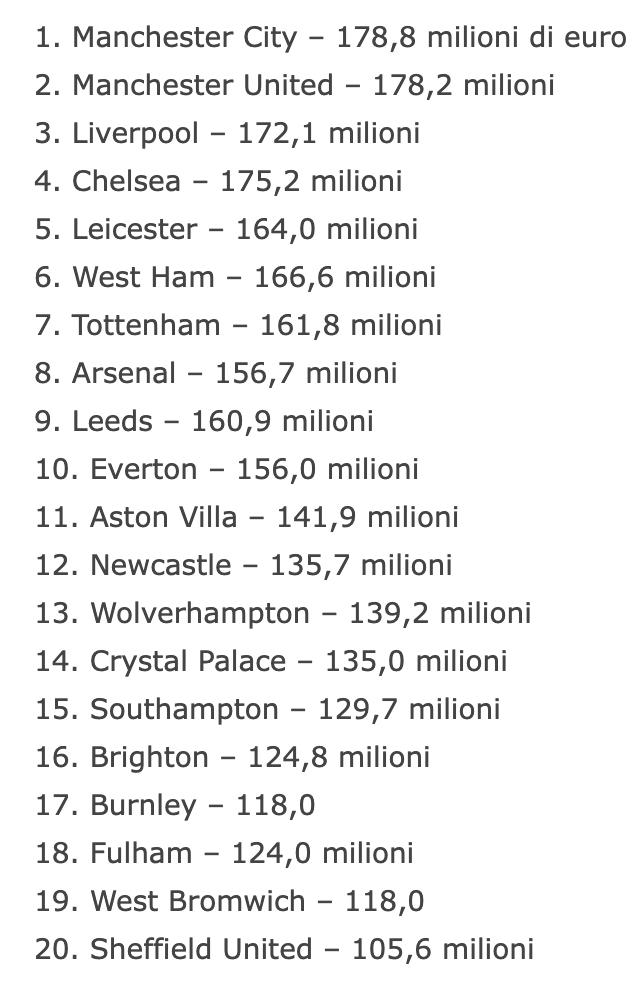
\includegraphics[width=.35\textwidth]{img/diritti_tv_pl.png} \label{diritti_tv_pl}} \quad
    \subfloat[][Incassi Diritti TV Serie A]
    {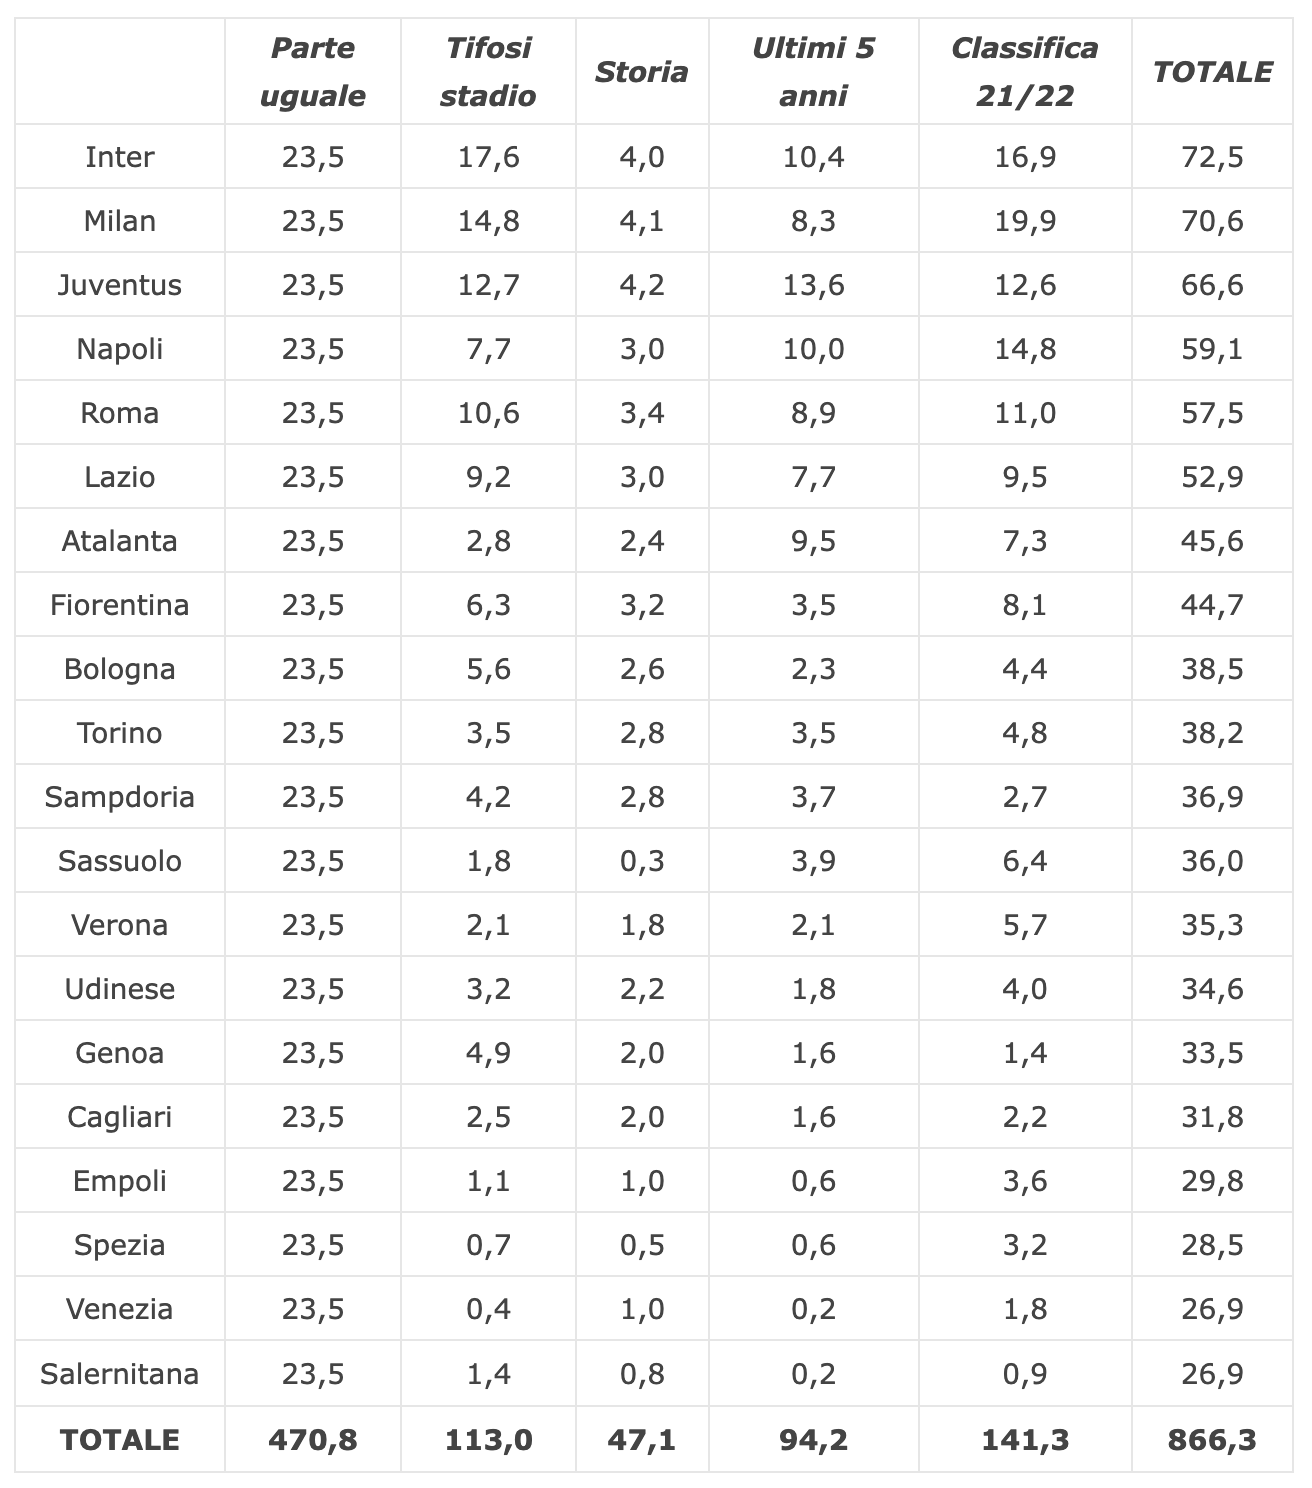
\includegraphics[width=.35\textwidth]{img/diritti_tv_SA.png} \label{diritti_tv_SA}}
    \caption{Comparazione incassi Diritti TV}
    \label{comp_diritti_tv}  
\end{figure}
Questi due fattori molto importanti permettono alla \emph{Premier League} di essere uno dei campionati pi\'u spettacolari e seguiti al mondo anche se 
il ricambio di vincitori non \'e ampissimo, ma sicuramente meglio di altri campionati.\newline
Vi \'e per\'o un ulteriore criticit\'a nata in seguito allo sviluppo del \emph{FFP}: la situazione delle \textbf{plusvalenze fittizie}.
Il sistema alla base non \'e assolutamente malevolo, dato che consiste semplicemente nel vendere un giocatore ad un prezzo maggiore rispetto
alla quota di ammortamento residua iscritta a bilancio, se la prima \'e appunto superiore si crea plusvalenza mentre se \'e minore una 
minusvalenza, come accade anche per le immobilizzazioni all'interno di una azienda di produzione. Volendo utilizzare un esempio numerico il 
calciatore Gonzalo Higuain, passando dal Napoli alla Juventus per la cifra di 90 milioni di euro ha generato alla squadra campana una plusvalenza
di circa 86 milioni di euro\footnote{Calcio e Finanza: https://www.calcioefinanza.it/2022/01/29/classifica-plusvalenze-record-serie-a-vlahovic-lukaku/}, 
dato che il contratto del calciatore era prossimo alla scadenza e quindi la quota rimanente a bilancio del suo ammortamento era molto bassa. 
Il problema nasce nel momento in cui queste plusvalenze vengono gonfiate ed utilizzate per sistemare i bilanci delle societ\'a, diventando 
appunto plusvalenze fittizie, perch\'e il valore di vendita in realt\'a non \'e effettivamente quello ceh \'e stato pagato. Il nostro campionato
\'e recentemente passato sotto la lente di ingrandimento degli inquirenti a causa di alcune operazioni sospette. Nel mirino sono finite alcune societ\'a
del massimo campionato tra cui Juventus, Napoli e Genoa ma anche societ\'a pi\'u modeste come Pro Vercelli e Pisa\footnote{SportMediaset: https://www.sportmediaset.mediaset.it/calcio/seriea/plusvalenze-la-figc-ha-trovato-la-formula-per-smascherare-le-valutazioni-fittizie\_48175965-202202k.shtml}. L'accusa \'e quindi di 
aver sostanzialmente falsificato i prezzi di vendita o di acquisto di alcuni calciatori in modo da facilitare il pareggio di bilancio.
In particolare alla squadra torinese si contestano circa 60 milioni di euro ricavati da valutazioni errate durante scambi di calciatori, mentre per 
il Napoli il problema principale riguarda l'operazione che ha portato in Italia Victor Osimhen, pagato poco pi\'u di 70 milioni, ma il suo reale 
valore si aggira in torno ai 52; nell'operazione sono poi stati aggiunti degli scambi con alcuni calciatori delle giovanili del Napoli il cui
valore \'e stato completamente ribaltato, passando da cifre sotto al milione a prezzi poco sotto i 10 milioni di euro. In tutto questo per\'o
le autorit\'a hanno le mani legate perch\'e sia in questo caso che in altri (l'utilizzo delle plusvalenze fittizie \'e iniziato alcuni anni fa)
non \'e possibile identificare un metodo univoco per la valutazione dei calciatori, rendendo quindi impossibile giudicare una societ1\'a
colpevole di aver gonfiato i valori di un cartellino. Ovviamente tutti sanno che nella pratica questo metodo viene utilizzato di continuo,
ma in termini legali non si pu\'o fare nulla.\newline
\chapter{La SuperLega: una nuova idea per salvare il mondo del calcio}
Nell'ultima parte di questo elaborato si andr\'a ad analizzare quella che viene definita una possibile soluzione a tutta questa situazione di 
instabilit\'a economica e che, secondo i principali sostenitori del progetto, andrebbe a risolvere l'elevata quantit\'a di debito 
che si \'e generata all'interno del calcio europeo.
La volont\'a di creare una \textbf{SuperLega} \'e, in realt\'a, sempre esistita. A partire dagli anni 80 e in modo sistematico ogni 10/15 
anni, alcune tra le figure pi\'u influenti nel panorama calcistico, avanzavano una proposta con la finalit\'a di creare una sola competizione che,
in un modo o in un altro, racchiudesse le squadre pi\'u forti (economicamente e sul piano del calcio giocato).\newline
La prima proposta della creazione di una SuperLega fu avanzata nel 1987 dall'allora presidente del Milan, Silvio Berlusconi, dal presidente
del Real Madrid Ramon Mendoza e dal segretario dei Glasgow Rangers Campbell Ogilvie\footnote{Wikipedia: \newline https://en.wikipedia.org/wiki/Proposals\_for\_a\_European\_Super\_League\_in\_association\_football}.
Il loro pensiero si basava sul fatto che l'attuale concezione della \emph{Champions League} fosse obsoleta, perci\'o era necessaria una riforma:
una competizione a girone unico basata sul metodo \emph{round-robin}, dove una squadra affronta obbligatoriamente tutte le squadre del girone. 
In questo modo sarebbe stato possibile incrementare i guadagni dai diritti televisivi dato che, secondo l'opinione del gruppo che aveva 
avanzato la proposta, questa nuovo format avrebbe generato un maggiore \emph{appeal} e generato un incremento di entrate per i club che 
ne avrebbero fatto parte. L'idea finale venne proposta alla UEFA nel 1990 ma fu immediatamente rigettata l'anno successivo, applicando anche 
sanzioni al Milan e al Real Madrid. Anche se la riforma non and\'o in porto, la Federazione decise comunque che sarebbe stato necessario modificare
qualcosa all'interno della competizione, furono introdotti quarti di finale semifinali e due gruppi di qualificazione all'italiana\footnote{Il girone all'italiana è una particolare formula delle competizioni con più di due partecipanti, che prevede lo svolgimento di incontri diretti tra tutti i partecipanti (intesi come individui oppure squadre) in tutti gli abbinamenti possibili}
di quattro squadre ciascuna. Ci f\'u anche un grosso \emph{rebrand} della competizione, con la decisione di registrare un logo e un inno.\newline
Nel 1999 vi f\'u un secondo tentativo di istituire una SuperLega, ovviamente si concluse con lo stesso epilogo della precedente: proposta 
ritirata a causa di una minaccia di applicazione di sanzioni da parte della UEFA. La situazione per\'o stava cambiando in qualche modo: 
stava nascendo una volont\'a sempre maggiore di attuare una corposa riforma nel calcio europeo. Quest\'a volont\'a raggiunse il culmine
nel 2021, con l'ultimissima proposta supportata questa volta dai 12 maggiori club di Inghiterra, Spagna e Italia. 
\section{Definizione e struttura}
Il 18 Aprile 2021, tramite un comunicato stampa, veniva annunciata la volont\'a di istituire una SuperLega con 20 club partecipanti e i 12 club
che avanzavano la proposta considerati come fondatori. La struttura della competizione era molto semplice: 
\begin{itemize}
    \item Una competizione infrasettimanale a cadenza annuale composta da 20 squadre, divise in due gironi da 10;
    \item Una prima fase "all’italiana" con partite di andata e ritorno fra squadre dello stesso girone
    \item Segue, poi, una fase a eliminazione diretta che coinvolge soltanto 10 squadre. Le prime tre di ogni 
    girone direttamente ai quarti di finale assieme alle vincenti degli spareggi fra le quarte e le quinte classificate;
    \item Gli accoppiamenti dei quarti sono determinati dalla classifica dei due gironi (prima di un girone contro la vincente 
    dello spareggio quarta/quinta dell’altro, seconda contro terza, ecc.). La finale in gara secca su campo neutro. 
    18 le partite garantite a ciascuna partecipante;
    \item La Superlega si disputa durante la normale stagione calcistica e si pone quindi come alternativa alla Champions League, 
    con gare infrasettimanali, ad eccezione della finale prevista nel weekend.
\end{itemize}
L'idea, per\'o, cos\'i come \'e stata avanzata in prima istanza era effettivamente considerabile come una volont\'a di voler istituire 
una campionato elitario in cui solo i pi\'u ricchi potessero partecipare, a discapito quindi dei meno abbienti. Il primo progetto infatti non prevedeva
alcun tipo di retrocessioni e promozioni, andando di fatto a creare un blocco di squadre che si sarebbero continuamente affrontate tra di loro
escludendo a priori tutte le altre. Un secondo aspetto importante che rendeva molto allettante la possibile nascita di questa nuova competizione
\'e la parte economica. Il principale finanziatore sarebbe stato \textbf{JPMorgan}, tramite un prestito di 3.5 miliardi di dollari da restituire
in 15 mesi. Una parte di quella cifra sarebbe servita per i costi di orgnizzazione, mentre i restanti sarebbero stati distribuiti come premi per i partecipanti,
con cifre dai 55 fino ai 250 milioni di euro all'anno\footnote{SkySport: https://sport.sky.it/calcio/2022/04/19/superlega-calcio-un-anno-dopo\#05}. 
Paradossalmente, in Italia, il vincitore del campionato riceve poco pi\'u di 30 milioni di euro mentre in Inghilterra la situazione migliora 
leggermente, con un premio per la squadra vincitrice di circa 70 milioni di sterline\footnote{Il Sole 24 Ore: https://www.ilsole24ore.com/art/lo-scudetto-regala-milan-27-milioni-introiti-ma-premier-e-lontanissima-AEZwCaaB}. 
Le cifre che questa nuova SuperLega mette sul piatto, per\'o, sono decisamente pi\'u allettanti, sopratutto per squadre come Inter, 
Milan oppure Atletico Madrid che negli ultimi anni sono usciti dai riflettori internazionali, vedendosi quindi diminuire gli incassi.\newline
Questa prima proposta di rivoluzione ha sconvolto totalmente il mondo del calcio e non solo, dato che anche leader politici e persone esterne
a questo ambito hanno voluto dare la loro opinione\footnote{Un maggiore approfondimento verr\'a effettuato successivamente}; ed \'e forse per 
questo che il progetto non ha avuto per nulla il successo sperato, andando di fatto a sgretolarsi in sole 48 ore. La volont\'a di 
cambiare per\'o non \'e stata spenta, tanto che nei primi mesi del 2022 \'e stato presentato un nuovo progetto, decisamente pi\'u inclusivo e 
meno elitario:
\begin{itemize}
    \item Saranno presenti promozioni e retrocessioni, andando quindi ad eliminare il problema da parte di altre squadre di entrare nella competizione;
    \item Saranno presenti 2 gironi da 20 squadre l'uno, andando ad ampliare il \emph{roster} di squadre partecipanti.
\end{itemize} 
Questi pochi e sintetici punti potrebbero di fatto portare ad una rivalutazione del progetto, che attualmente non \'e stata neanche presa in
considerazione. 
La volont\'a di mettere in pratica un progetto cos\'i rivoluzionario e innovativo ma allo stesso tempo molto lontano dalle attuali dinamiche del
mondo del calcio, non nasce sicuramente in un anno. Anche per quanto riguarda ques'ultimo progetto, quello che sulla carta sembra il pi\'u
possibile ad avverarsi, \textbf{le origini risalgono almeno al 2016}. Sempre grazie all'associzione \emph{Football Leaks} sappiamo che \'e avvenuto un incontro tra i 
rappresentanti di societ\'a come Real Madrid, Juventus e Bayern Monaco all'incirca il 31 Marzo del 2016 in un albergo a Zurigo\footnote{https://www.calcioefinanza.it/2018/11/02/football-leaks-e-superlega-europea-piani-big/}. Il programma
dell'incontro era ovviamente la volont\'a di creare un campionato elitario, a invito, in cui le migliori squadre d'Europa si sarebbero scontrare tra loro. 
Il motivo principale che ha spinto questi club a volere un qualcosa come la SuperLega \'e indubbiamente legato all'enorme deficit
di bilancio che non riescono (o non vogliono) eliminare e che, tramite questa nuova competizione ed i relativi fondi, in pochi anni riuscirebbero a colmare.
Se si volesse stilare una lista dei club che hanno proposto l'idea di SuperLega nell'Aprile del 2021, si potrebbe notare come tutti, escluso 
il Real Madrid registrino importanti perdite. La tabella sottostante\footnote{Calcio e Finanza: https://www.calcioefinanza.it/2022/03/27/classifica-perdite-bilancio-superlega/} lo mostra in modo immediato:\newpage
\begin{table}
    \begin{tabularx}{\textwidth}{XX}
        \toprule
        \textbf{Squadra} & \textbf{Risultato aggregato 19/20 - 20/21} \\
        \midrule
        Barcellona & 578 milioni di euro \\
        \midrule
        Inter & 348 milioni di euro \\
        \midrule
        Juventus & 300 milioni di euro \\
        \midrule
        Milan & 291 milioni di euro \\
        \midrule
        Manchester City & 247 milioni di euro \\
        \midrule
        Arsenal & 192 milioni di euro \\
        \midrule
        Tottenham & 175 milioni di euro \\
        \midrule
        Manchester United & 134 milioni di euro \\
        \midrule
        Chelsea & 126 milioni di euro \\
        \midrule
        Atletico Madrid & 109,2 milioni di euro \\
        \midrule
        Liverpool & 51 milioni di euro \\
        \midrule
        Real Madrid & +1,5 milioni \\
        \bottomrule
    \end{tabularx}
    \caption{Tabella Perdite aggregate per i 12 club promotori dell'idea SuperLega}
    \label{tabella_ris_sl}
\end{table}
In questo modo i conti sono presto fatti: se ipoteticamente il vincitore della SuperLega ricevesse all'incirca 250 milioni di euro, pi\'u
della met\'a delle squadre nella tabella avrebbero risolto il problema del debito. Ovviamente il calcolo \'e un po' semplicistico ma non 
si discosta molto dalla realt\'a.
\section{Reazione di Media e persone}
Lo notizia della volont\'a di creare una SuperLega ha inevitabilmente scosso tutto il mondo del calcio e non solo. Come gi\'a anticipato prima 
tutte le figure di potere del mondo ma sopratutto europee hanno voluto dare la loro opinione riguardo la necessit\'a o meno di creare questa nuova competizione.
Inanzitutto la prima risposta arriv\'o dalla UEFA e dal suo presidente Aleksander Čeferin che ha fin da subito condannato la proposta, paragonando
addirittura i club ad un gruppo di \textbf{terrapiattisti}: \begin{quote}\small \'E strano però che vogliano un loro torneo, ma contemporaneamente vogliano giocare nel nostro, 
di torneo. Ad ogni modo, per me questo è un argomento chiuso. Magari qualcuno vuole insistere, ma c’è anche qualcuno che continua a insistere sul fatto 
che la terra sia piatta.\footnote{Intervista di Aleksander Čeferin a SkySport}\end{quote} Con queste parole molto forti \'e indubbiamente comprensibile come la federazione europea non accetter\'a mai 
ed in alcun modo nemmeno un compromesso con questi club. Ma riusciranno davvero a non cedere?\newline
Oltre al presidente della UEFA anche molti calciatori ed ex hanno voluto dare la loro opinione: \textbf{Ander Herrera} attuale calciatore del PSG ha commentato: 
\begin{quote}\small Mi sono innamorato del calcio popolare, del calcio dei tifosi, con il sogno di vedere la squadra del mio cuore sfidare i più grandi. Se questo progetto 
della Superlega proseguirà, questo sogno è destinato a finire. Il desiderio dei tifosi delle squadre che non sono ai vertici di vedere i loro team battere 
sul campo i più grandi, è spento.\end{quote} Prosegue poi \textbf{Lucas Podolski} (impiegato attualmente nel campionato turco): \begin{quote}\small La Superlega è un insulto verso quello 
in cui credo: il calcio è felicità, liberta, passione, tifosi, ed è per tutti. Questo progetto mi disgusta, non è giusto e sono veramente contrariato di vedere coinvolti 
club di cui ho fatto parte. Dobbiamo combattere tutto questo.\end{quote}
Infine anche l'ex bandiera del Manchester United \textbf{Gary Neville} \'e sulla stessa linea dei suoi colleghi: \begin{quote}\small Una vergogna assoluta, sono disgustato. E' pura avidità,
i proprietari di questi club sono degli impostori, anche quelli dello United per il quale faccio il tifo da 40 anni. Non hanno nulla a che fare con il 
calcio in questo Paese, dove c'è una storia lunga 100 anni di tifosi che hanno vissuto e amato i loro club. Bisogna penalizzare questi club, subito. 
Farli retrocedere e togliere loro tutti i soldi.\end{quote}
Tutti questi sono Tweet\footnote{SkySport: https://sport.sky.it/calcio/2021/04/19/superlega-reazioni-calciatori-contro\#09} pubblicati direttamente dai diretti interessati, 
che sono voluti scendere in campo in prima persona per cercare di evitare che si venisse a creare una possibile SuperLega.
Un altro episodio che ha dato un forte scossone all'opinione pubblica \'e arrivato dal Liverpool e dai suoi tifosi: la squadra inglese era
tra le 12 fondatrici del progetto SuperLega, ma appena la notizia \'e stata resa pubblica, i suoi tifosi pi\'u fedeli, che compongono la curva 
\emph{Kop}\footnote{Una della pi\'u fedeli del panorama calcistico}, si sono letteralmente rivoltati. Anche loro tramite 
Twitter scrivono: \begin{quote}\small Noi, insieme agli altri gruppi coinvolti, rimuoveremo le bandiere dalla Kop. Riteniamo di non poter più dare
il nostro sostegno ad un club che pone l'avidità finanziaria al di sopra dell'integrità del gioco.\end{quote}
Questa forte disapprovazione ha fatto immediatamente cambiare idea al club, che \'e stato infatti tra i primi a ritirarsi dalla proposta, seguito
poi da molti altri club per paura di forti ripercussioni da parte della UEFA.\newline
In seguito a questa prima "ondata" di opionioni da parte di personaggi influenti del mondo del calcio, \'e venuto il turno dei leader politici.
Anche se nessuno si aspetterebbe una loro opinione, dato che teoricamente il calcio non ha nulla a che vedere con la politica, molti tra i pi\'u 
famosi Capi di Stato sono intervenuti sulla vicenda: da \textbf{Boris Johnson} fino ad \textbf{Emmanuel Macron}, passando da Mario Draghi, tutti loro hanno condannato
la volont\'a di creare la SuperLega e in alcuni casi minacciando sanzioni ai calciatori delle squadre promotrici. Per esempio il Primo 
Ministro inglese ha dichiarato che <<non escludo di impedire ai giocatori che parteciperanno alla Super League di ricevere visti o di ritirare i fondi per le forze dell'ordine che dovranno vigilare sulle partite>>
\footnote{AGI: https://www.agi.it/sport/calcio/news/2021-04-20/super-league-boris-johnson-alza-muro-cerca-dialogo-12248117/}. In Francia, invece, l'opinione del Capo di Stato viene riassunta in queste poche parole:
<<mette a repentaglio il principio di solidarietà e di meritocrazia nello sport>>\footnote{Corriere: https://www.corriere.it/sport/21\_aprile\_18/macron-contro-superlega-progetto-sbagliato-francia-sosterra-uefa-7f267254-a06f-11eb-b0fa-564f55184e78.shtml};
infine l'attuale Presidente del Consiglio dei Ministri italiano ha un idea simile a quella del suo pari francese: \begin{quote}
    \small Il governo segue con attenzione il dibattito intorno al progetto della Superlega calcio e sostiene con determinazione le posizioni delle autorità calcistiche italiane ed europee per preservare le competizioni nazionali, i valori meritocratici e la funzione sociale dello sport.\footnote{SkySport: https://sport.sky.it/calcio/2021/04/19/mario-draghi-superlega-europea-calcio}
\end{quote} 
Nel caso francese, per\'o, \'e necessario fare una piccola aggiunta: l'interesse del Primo Ministro di impedire la creazione di una SuperLega
\'e indubbiamente legata alla sua forte "relazione" con la squadra pi\'u importante del Paese e molto influente a livello mondiale: il Paris Saint Germain.
Il primo caso eclatante che ha lasciato molti appassionati perplessi \'e accaduto durante le trattive per il rinnovo di contratto di pochi mesi fa del calciatore
Kylian Mbapp\'e, appunto militante nella squadra parigina. Quest'ultimo non era del tutto convinto di continuare a giocare in Francia, forse 
a per le continue delusioni sportive della sua squadra oppure semplicemente per una voglia di cambiare aria; il Real Madrid colse quindi l'occasione e offr\'i
sul piatto uni cifra \emph{monstre} di 180 milioni di euro alla firma del contratto e circa 40 milioni come stipendio\footnote{Calciomercato.com: https://www.calciomercato.com/news/real-madrid-la-cifra-offerta-a-mbappe-e-l-ostacolo-dei-diritti-d-21776}.
Qualunque giocatore, posto di fronte a una scelta di quel tipo, non avrebbe atteso 1 minuto ad accettare, ed \'e qu\'i che entra in gioco la politica: Emmanuel Macron 
stesso ha ammesso di aver telefonato al giocatore francese "consigliandogli di rimanere in Francia"\footnote{SkySport: https://sport.sky.it/calcio/ligue-1/2022/06/04/macron-mbappe-psg-news}.
Ovviamente poche settimane dopo la telefonata, il calciatore decise di rinnovare alle cifre che tutt'ora rimangono tra le pi\'u alte mai
offerte ad un calciatore in tutta la storia: 130 milioni di euro alla firma del contratto e 30 milioni di euro all'anno\footnote{Gazzetta dello Sport: https://www.gazzetta.it/Calciomercato/21-05-2022/mbappe-psg-sorpassa-real-gia-stasera-annuncio-rinnovo-440611920512.shtml}. Macron ovviamente 
nega di aver in qualche modo costretto il calciatore a rimanere, affermando come <<il ruolo di un presidente è quello di difendere il Paese>>, ma 
a molti rimarr\'a il dubbio che non sia stato solo quello. \'E emerso poi un secondo episodio legato a Macron e il PSG: il presidente francese ha ammesso pubblicamente
il proprio interesse verso la trattativa, ancora non ufficiale, che porterebbe l'ex calciatore e brillante allenatore Zinedine Zidane sulla 
panchina del club parigino. Anche in questo caso sembra che il calcio diventi un affare di stato.\newline
Questi ultimi due esempi possono sostenere la tesi sulla possibilit\'a che il calcio sia diventato un'economia talmente vasta e che raccoglie
l'interesse di talmente tanti settori diversi, che anche gli Stati devono fare in modo che questo "asset" generi pi\'u entrate possibili all'interno
del proprio Paese.
\section{La SuperLega \'e necessaria?}
Quest'ultima sezione cercher\'a di racchiudere tutte le idee e le opinioni elencate nelle sezioni precedenti per capire, in ultima battuta,
se questa SuperLega sia davvero necessaria per salvare il calcio mondiale, oppure sia semplicemente un capriccio di alcuni dirigenti
ricchi e potenti.\newline
Se si analizza la situazione in modo pi\'u neutro e senza farsi influenzare dalle, comprensibilissime, opinioni delle varie figure del mondo 
dello sport e non solo, \'e possibile concepire come l'idea della SuperLega non sia del tutto sbagliata e discriminatoria.
Il punto focale \'e che, come si suol dire, i tempi cambiano ed \'e impossibile limitare il cambiamento. Si \'e arrivati ad un punto di non ritorno
causato in parte dalle societ\'a stesse che, come si ha avuto modo di elaborare lungo il percorso di questa trattazione, non si sono fatte scrupoli 
a spendere pi\'u del dovuto, e in parte uguale anche dalla federazione stessa, che ha giustamente voluto applicare delle regole per frenare comportamenti antisportivi 
ma sopratutto illegali, ma che alla fine hanno solo danneggiato l'immagine dello sport. Dato che la UEFA, tramite il FFP, non \'e riuscita
ad alleggerire il problema derivato da anni di controlli inesistenti oppure troppo blandi, le societ\'a stesse hanno sviluppato una loro soluzione.
Un secondo punto, forse di natura leggermente pi\'u cinica, \'e che le categorie sono sempre esistite. Sicuramente vietare a priori alle squadre
minori, oppure che basano la loro idea su un progetto a lungo termine di partecipare ad una possibile SuperLega \'e sbagliato, 
ma non l'idea in s\'e di competizione. Attualmente nei vari campionati si affrontano squadre con un divario tecnico estremamente elevato, 
sopratutto in Paesi come Francia o Inghilterra, e spesso il risultato finale assomiglia quasi pi\'u ad una partita di tennis rispetto ad una
di calcio. Per questo motivo la creazione di una SuperLega, diminuirebbe il tasso tecnico di alcuni campionati, facilitando la crescita di alcune realt\'a 
che non si troverebbero pi\'u ad affrontare strapotenze con centinaia di milioni di euro di investimenti ogni anno, ma square pi\'u simili al loro livello
aprendo maggiori possibilit\'a ad una crescita pi\'u rapida. Utilizzando un esempio pratico, se nel campionato di Serie A le squadre che originariamente avevano
aderito al progetto iniziale partecipassero davvero ad una SuperLega, sarebbero maggiormente inclini a schierare giocatori pi\'u giovani oppure
calciatori non propriamente titolari, andando a diminuire la differenza tecnica con le squadre minori. Una partita come Juventus-Sampdoria, giocata
ad armi pari darebbe sicuramente maggiore soddisfazione, sopratutto ai tifosi Liguri, che riuscirebbero a vedere la loro squadra che notoriamente
affanna contro una compagine come la Juventus, magari anche ad ambire alla conquista dei 3 punti. Ovviamente anche per la Juventus ci sarebbero
aspetti positivi dato che potrebbero dare la chance a calciatori pi\'u giovani di giocare partite con altri professionisti, contribuendo alla loro 
crescita ma anche a quella del calcio internazionale, che in particolare per l'Italia ha necessit\'a di un grande progetto per tornare ai vertici.
Un terzo punto a sostegno della SuperLega riguarda il paragone che spesso \'e stato fatto con il modello americano. In America i campionati di NBA\footnote{Campionato di Basket}
ed NFL\footnote{Campionato di Football Americano} generano introiti nel primo caso di 8 miliardi di dollari\footnote{Forbes, dati del 2019} e di addirittura
15 miliardi per il campionato di Football\footnote{Il Sole 24 Ore: https://www.ilsole24ore.com/art/super-bowl-nfl-vicina-meta-15-miliardi-d-incassi-AEI3JXDB}.
Il problema sorge per\'o se si analizza il numero di spettatori coinvolti: la finale di Champions League 2018/2019 \'e stata vista da un totale di 
circa 94 milioni di persone\footnote{Dati non completi} contro i circa 150 relativi alla finale \emph{Super Bowl}\footnote{Calcio e Finanza: https://www.calcioefinanza.it/2020/08/23/champions-league-vs-super-bowl-chi-vale-di-piu-il-confronto/}. 
I numeri degli spettatori sono molto simili ma allo stesso tempo gli incassi sono incredibilmente distanti: 2.853 miliardi di euro per la competizione calcistica e 
circa 17 miliardi di dollari per il campionato di football. Utilizzando quindi un modello come quello americano, salta subito all'occhio come 
il modello americano a fronte dello stesso numero di persone che usufruiscono del "servizio" generi decisamente pi\'u introiti. Il motivo che pi\'u 
di tutti gli altri impedisce l'effettiva possibilit\'a di realizzare qualcosa simile a quel modello, \'e la diversa idea di sport che c\'e tra
Europa e America: nel primo caso abbiamo una concezione maggiormente legata al risultato e alla volont\'a di voler vincere, senza considerare quindi
nessun fattore esterno al campo come possono essere tifosi o sponsor; ovviamente sempre in modo relativo dato che questi due fattori compongono la 
maggior percentuale delle entrate di un club\footnote{Vedasi capitolo 1}; nel secondo caso, invece, il risultato sportivo passa completamente in secondo piano,
lasciando spazio ad una mentalit\'a completamente indirizzata allo spettacolo. Nel nuovo continente tutte le partite, che siano calcio, basket 
oppure football americano hanno come fine principale quello di soddisfare la persona che sta guardando, che sia essa in TV oppure dal vivo;
i \emph{match} sono dei veri e propri spettacoli, con momenti deidicati totalmente al divertimento. Durante la finale del Super Bowl, infatti,
\'e presente un occasione che prende il nome di \emph{Halftime Show} dedicato all'esibizione di artisti di calibro internazionale come per esempio 
Katy Perry, Madonna o i Coldplay. Oltre a questo, sui maxi-schermi presenti allo stadio vengono riprodotti in continuazione spot pubblicitari, 
e per poche decine di secondi le societ\'a sono disposte a pagare milioni di dollari. Per esempio, nel 2021, il costo per uno spot di venti secondi 
era di circa 5.6 milioni di dollari\footnote{Fonte dati: Calcio e Finanza}.\newline
Avendo quindi prova di come i due diversi continenti abbiano una idea di sport diametralmente opposta, \'e facilmente intuibile il motivo di tutta questa riluttanza
verso questo nuovo progetto. Il punto su cui bisogna soffermarsi, per\'o, \'e il fatto che, se si vuole salvare il sistema calcio, \'e necessario
rivedere la propria posizione e le proprie idee, per dare priorit\'a ad un qualcosa che permetter\'a ad uno degli sport pi\'u seguiti del mondo
di sopravvivere. Nella sezione precedente molti calciatori ribadiscono il concetto che il calcio deve essere dei tifosi; queste poche parole
sono diventate uno slogan per chi ha assunto una posizione contro la Superlega. Ma davvero esiste ancora il calcio "dei tifosi"? Anche 
la UEFA stessa porta avanti questa idea, di come il calcio non debba escludere nessuno e che i valori dello sport non hanno nulla a che fare con la 
Superlega; la stessa UEFA che \'e stata praticamente colta sul fatto ad operare in modo illecito con altri club che tutt'ora giocano tranquillamente
le competizioni europee. Le colpe della UEFA, per\'o, non si fermano tuttavia solo a quello: il piano di utilizzare il Fair Play Finanziario come 
strumento per riportare il calcio ad una tranquillit\'a economica, \'e sostanzialmente fallito, ed \'e per questo motivo, dopo poco pi\'u di 
10 anni di utilizzo di questo sistema per il controllo finanzario ed economico delle squadre, la federazione ha ideato un nuovo sistema, 
casualmente ispirato ad un modello americano: il \textbf{\emph{Salary Cap}}. Questo modello, gi\'a ampiamente in uso nel massimo campionato di 
basket americano ma anche nella Liga spagnola\footnote{Massimo campionato di calcio spagnolo}, consiste essenzialmente in una percentuale di denaro che i
club possono utilizzare per pagare lo stipendio dei propri tesserati (calciatori e non) in rapporto al proprio fatturato. In NBA il tetto 
massimo spendibile \'e fondamentalmente uguale per tutte le squadre e fissato ad una cifra di circa 112 milioni di dollari\footnote{Dunkest.com: https://www.dunkest.com/it/nba/notizie/mercato/12921/nba-salary-cap-come-funziona};
mentre per quanto riguarda il campionato spagnolo viene calcolato tramite una percentuale in base al fatturato. La federazione europea, vorebbe 
utilizzare questa linea di ragionamento anche per quanto riguarda le competizioni europee, pi\'u precisamente una società potrà spendere al massimo il 70\% dei suoi ricavi, 
suddivisi nel 90\% la prossima stagione calcistica e l'80\% in quella successiva\footnote{SkySport: https://sport.sky.it/calcio/champions-league/2022/03/28/eca-qualificazione-champions-league-ranking}.\newline
Terminando questa sezione cercando di rispondere alla domanda posta nel titolo, \textbf{la Superlega \'e davvero necessaria?}, la risposta che si potrebbe
dare osservando i dati presentati \'e che s\'i, lo sarebbe. 
\chapter{Conclusione Finale}
\end{interlinea}
\end{document}

